\documentclass{beamer}

\title{Model Antrian \textit{Multi-Server:} M/M/c}
\subtitle{dengan Pengantar Model Stokastik dan Teori Antrian \\ dengan R dan QtsPlus \\ (Revisi)}
\author{Bisma Rohpanca Joyosumarto (2106635581)}
\institute{Departemen Matematika FMIPA UI \\ Universitas Indonesia}
\date{
    November 2024

    Riset Operasi
    
    Tahun Ajaran 2024/2025 Semester Ganjil
}

% === bismastyle.sty ===
%\usetheme{Copenhagen}

\AtBeginSection[]
{
  \begin{frame}{Daftar isi keseluruhan}
    \tableofcontents[currentsection]
  \end{frame}
}

\AtBeginSubsection[]{
  \frame<beamer>{ 
    \frametitle{Daftar isi di bab}   

\tableofcontents[currentsection,currentsubsection,sectionstyle=show/hide,subsectionstyle=show/shaded/hide,subsubsectionstyle=show/show/shaded/shaded]}
}
% sumber: https://tex.stackexchange.com/questions/434088/beamer-toc-on-each-subsection

\addtobeamertemplate{navigation symbols}{}{%
    \usebeamerfont{footline}%
    \usebeamercolor[fg]{footline}%
    \hspace{1em}%
    \insertframenumber/\inserttotalframenumber
}

\newcommand{\pars}[1]{\left(#1\right)}
\newcommand{\brackets}[1]{\left[#1\right]}
\newcommand{\braces}[1]{\left\{#1\right\}}

\usepackage{hyperref}
\usepackage{graphicx}
\usepackage{amsmath}
\usepackage{enumerate}
\usepackage{systeme}
\sysdelim..

\usepackage{minted}
% === akhir bismastyle.sty ===

\begin{document}

\frame{\titlepage}

\begin{frame}{Daftar isi keseluruhan}
    \tableofcontents
\end{frame}

\section[Pengantar Model Stokastik dan Teori Antrian. dengan praktik di R]{Pengantar Model Stokastik dan Teori Antrian \\ dengan praktik di R}

\begin{frame}{\textit{Overview:} Teori Antrian dan Model Stokastik}
    \begin{itemize}
        \item Dalam suatu \textbf{antrian \textit{(queue)}}, orang bisa masuk mengantri, dilayani, kemudian meninggalkan antrian
        \item Apabila ada beberapa pelayan, tiap baris/pelayan disebut \textit{server}, sehingga secara keseluruhan, terdapat satu antrian dengan sejumlah \textit{server}
        \item Pada dasarnya, proses mengantri bisa dimodel dengan melihat dua aspek: proses datangnya orang, dan proses perginya orang
        \item Di kuliah Pengantar Sains Data (Metode Statistika), kita sudah kenal \textbf{distribusi Poisson} yang memodelkan probabilitas banyaknya kemunculan dalam suatu satuan waktu, dalam yang namanya \textbf{proses Poisson}
        \item Baik datangnya orang maupun perginya orang, masing-masing bisa dimodelkan sebagai proses Poisson: datangnya orang sama saja kemunculan di pintu masuk, dan perginya orang sama saja kemunculan di pintu keluar
    \end{itemize}
\end{frame}

\begin{frame}{\textit{Overview:} Proses Poisson dan Rantai Markov}
    \begin{itemize}
        \item Sifat utama proses Poisson adalah \textbf{sifat Markov} atau \textbf{sifat \textit{memoryless:}} probabilitas kedatangan \textbf{hanya bergantung pada kondisi saat itu}, tidak pada kondisi di masa lalu
        \item Proses Poisson adalah contoh \textbf{rantai Markov waktu kontinu} atau \textbf{\textit{continuous-time Markov chain} (CTMC)}
        \item CTMC itu sendiri adalah perumuman dari \textbf{rantai Markov waktu diskrit} atau \textbf{\textit{discrete-time Markov chain} (DTMC)}
        \item Agar lebih paham dasar statistik untuk teori antrian, termasuk mengapa distribusi Poisson dan distribusi eksponensial sering digunakan, mari kita bahas dari awal!
    \end{itemize}
\end{frame}

\subsection{Rantai Markov Waktu Diskrit (DTMC)}

\begin{frame}{Definisi DTMC}
    Secara umum, dalam suatu rantai Markov, ada sejumlah kemungkinan "keadaan" \textit{(state)}, ada waktu, dan ada probabilitas berpindah dari suatu \textit{state} ke \textit{state} lain di tiap waktu berikutnya.

    Suatu DTMC, misal ditulis \( \braces{X_t} \), terdiri dari
    \begin{itemize}
        \item Suatu \textit{state space} atau himpunan \textit{state}, misal \( S \), 
        %berisi semua "keadaan" \textit{(state)} yang mungkin
        yang terhitung (bisa berhingga)
        \item Himpunan indeks waktu, biasanya \( T = \braces{0, 1, 2, \dots} \)
        \item $X_t$ sebagai variabel acak untuk tiap \( t \in T \), yang nilainya bisa berupa \textit{state} apapun dari \( S \). Sehingga, \( \braces{X_t} \) adalah barisan variabel acak
    \end{itemize}
    dan memenuhi \textbf{sifat Markov} \textbf{(\textit{Markov property})} atau \textbf{\textit{memoryless property}} sebagai berikut:
    \begin{align*}
        \text{Pr}&\braces{X_{n+1} = j \, \mid \, X_0 = i_0, \, \dots \, X_{n-1} = i_{n-1}, X_n = i} \\
        &= \text{Pr}\braces{X_{n+1} = j \, \mid \, X_n = i}
    \end{align*}
    Artinya: probabilitas nilai \( X_t \) di waktu ke-\(\pars{n+1}\) hanya bergantung pada probabilitas di waktu ke-\(n\). Seolah-olah, tidak ada ingatan sama sekali tentang apa yang terjadi sebelum waktu ke-\(n\).

    %DTMC adalah contoh \textbf{proses stokastik \textit{(stochastic process)}}.
\end{frame}

\begin{frame}{DTMC stasioner}
    \begin{itemize}
        \item Kita bisa notasikan
        \[ P_{ij}^{n,n+1} = \text{Pr}\braces{X_{n+1} = j \, \mid \, X_n = i} \]
        yang disebut \textit{one-step transition probability}, dari \(X_n\) yang berada di \textit{state} \(i\) menjadi \(X_{n+1}\) yang berada di \textit{state} \(j\)
        \item Apabila nilai \(P_{ij}\) \textbf{tidak tergantung kapan}, maka rantai Markov disebut \textbf{stasioner}, dengan \textit{stationary transition probabilities}
        \item Dengan demikian, kita bisa menyusun \textbf{\textit{transition probability matrix} (TPM)} sebagai berikut, misalkan \(S=\braces{0,1,2,\dots}\):
        \[ P = \begin{pmatrix}
            P_{00} & P_{01} & P_{02} & \dots \\
            P_{10} & P_{11} & P_{12} & \dots \\
            \vdots & \vdots & \vdots & \ddots
        \end{pmatrix} \]
        dengan
        \[ P_{ij} = \text{Pr}\braces{X_{n+1} = j \, \mid \, X_n = i} \]
        sehingga baris ke-\(i\), kolom ke-\(j\) mengandung probabilitas transisi dari \textit{state} \(i\) ke \textit{state} \(j\).
    \end{itemize}
\end{frame}

\begin{frame}{Contoh DTMC stasioner: Semir Sepatu}
    Misalkan ada usaha kecil semir sepatu. Hanya ada satu pelayan dan dua kursi pelanggan.
    \begin{itemize}
        \item Apabila kedua kursi kosong, orang cenderung tidak sadar bahwa itu adalah tempat semir sepatu, sehingga tidak datang.
        \item Namun, ketika salah satu kursi terisi, probabilitas kursi lainnya ikut terisi menjadi dua kali lipat dari biasanya.
        \item Ketika ada dua pelanggan, probabilitas satu pelanggan selesai adalah empat kali probabilitas keduanya belum selesai.
        \item Misalkan juga, tidak mungkin dua pelanggan datang sekaligus ataupun selesai sekaligus, dan tidak mungkin selesainya satu orang langsung diikuti datangnya pelanggan baru.
    \end{itemize}

    Ada empat keadaan yang mungkin, misalnya \( S = \braces{0,1,2,3} \) sebagai berikut
    \begin{enumerate}
        \item[(0)] Kedua kursi kosong
        \item[(1)] Kursi pertama saja diisi
        \item[(2)] Kursi kedua saja diisi
        \item[(3)] Kedua kursi diisi
    \end{enumerate}
\end{frame}

\begin{frame}{TPM untuk Contoh DTMC}
    TPM dari situasi di atas adalah seperti berikut:
    \[ P = \begin{pmatrix}
        0.5 & 0.25 & 0.25 & 0 \\
        0.25 & 0.25 & 0 & 0.5 \\
        0.25 & 0 & 0.25 & 0.5 \\
        0 & 0.4 & 0.4 & 0.2
    \end{pmatrix} \]
    Perhatikan bahwa sumasi tiap baris adalah satu. Ini akibat sifat probabilitas. Dari suatu \textit{state} \(i\), dia bisa ke \textit{state} lainnya (atau bahkan tetap di \textit{state} yang sama) dengan probabilitas tiap kemungkinan ke \textit{state} \(j\) sesuai baris ke-\(i\).
\end{frame}

\begin{frame}{Diagram Transisi untuk Contoh DTMC}
    TPM bisa divisualisasikan sebagai \textbf{diagram transisi} atau \textbf{\textit{transition diagram}} sebagai berikut

    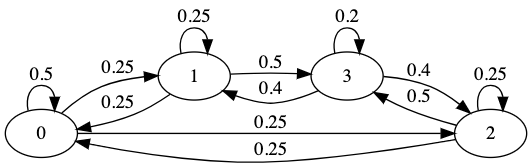
\includegraphics[scale=0.5]{gambar/contoh_dtmc.png}

    \begin{itemize}
        \item Tiap simpul melambangkan \textit{state}
        \item Tiap busur dari \(i\) ke \(j\) melambangkan transisi, dengan label \(P_{ij}\)
        \item Transisi dengan probabilitas nol tidak digambarkan
    \end{itemize}
    \textit{Fun fact:} rantai Markov adalah versi probabilistik dari automata hingga.
\end{frame}

\begin{frame}{Perbandingan: Diagram Transisi untuk Antrian}
    %Sedikit demi sedikit, kita coba lebih memahami teori antrian.
    Sebagai perbandingan dengan konsep antrian, perhatikan gambar berikut!

    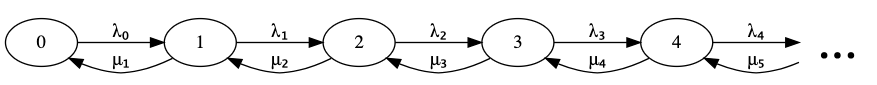
\includegraphics[scale=0.5]{gambar/diagram_transisi_antrian.png}

    Ini adalah diagram transisi yang umum dikenal untuk antrian.
    \begin{itemize}
        \item Himpunan \textit{state} \( S = \{ 0, 1, 2, 3, \dots \} \) menyatakan banyaknya orang (yang sedang mengantri) di antrian.
        \item Probabilitas \( P_{i,i+1} \), yaitu ketika banyaknya orang bertambah satu dari \( i \) (menjadi \( i+1 \) orang), ditulis \( \lambda_i \)
        \item Probabilitas \( P_{i,i-1} \), yaitu ketika banyaknya orang berkurang satu dari \( i \) (menjadi \( i-1 \) orang), ditulis \( \mu_i \)
    \end{itemize}
    Kita akan lihat nanti, notasi huruf \( \lambda \) tidak sembarangan dipilih.
\end{frame}

% Simulasi dan Analisis DTMC di R
\begin{frame}[fragile]{DTMC di R dengan \textit{package} markovchain}
    DTMC tergolong model stokastik (juga disebut proses stokastik) karena sifatnya yang probabilistik, sehingga menjadi pembahasan di ranah statistika (hingga menjadi kuliah Model Stokastik 1). Oleh karena itu, model stokastik seperti DTMC bisa disimulasikan di bahasa pemrograman R yang biasa digunakan oleh statistikawan. 
    
    Untuk DTMC, kita bisa gunakan \textit{package} markovchain:

\begin{minted}{r}
# install kalau belum
#install.packages("markovchain")

library("markovchain")
\end{minted}

    (Nanti akan ada \textit{package} khusus untuk simulasi antrian.)
\end{frame}

\begin{frame}[fragile]{Contoh DTMC di R}
    Kita bisa susun TPM dari contoh DTMC yang telah dibahas, sebagai berikut:

\begin{minted}{r}
mc1_P <- matrix(
  c(0.5,  0.25, 0.25, 0,
    0.25, 0.25, 0,    0.5,
    0.25, 0,    0.25, 0.5,
    0,    0.4,  0.4,  0.2),
  nrow = 4,
  byrow = TRUE
)
\end{minted}

Karena opsi \verb|byrow = TRUE|, matriks yang terbentuk akan seperti tertulis. Perhatikan bahwa dipasang \verb|nrow = 4| agar R tidak salah membaca data yang diberikan, yaitu agar matriks memiliki 4 (empat) baris.
\end{frame}

\begin{frame}[fragile]{Contoh DTMC di R}
    Setelah menyusun TPM, kita bisa mendefinisikan isi himpunan \(S\),

\begin{minted}{r}
mc1_states <- c("0", "1", "2", "3")
\end{minted}
    kemudian membuat objek \verb|markovchain| atau DTMC seperti berikut:

\begin{minted}{r}
mc1_obj <- new("markovchain",
               states = mc1_states,
               transitionMatrix = mc1_P)    
\end{minted}

    Informasi \textit{states} dan TPM bisa diperoleh kembali dengan mengetik nama objeknya:

\begin{minted}{r}
mc1_obj
\end{minted}

    Untuk memperoleh informasi \textit{states} saja, bisa digunakan fungsi \verb|states|

\begin{minted}{r}
states(mc1_obj)
\end{minted}

    Selain itu, diagram transisi juga bisa ditampilkan (lihat \textit{slide} berikutnya) dengan fungsi \verb|plot| seperti berikut.

\begin{minted}{r}
plot(mc1_obj)
\end{minted}
\end{frame}

\begin{frame}{Plot Diagram Transisi di R}
    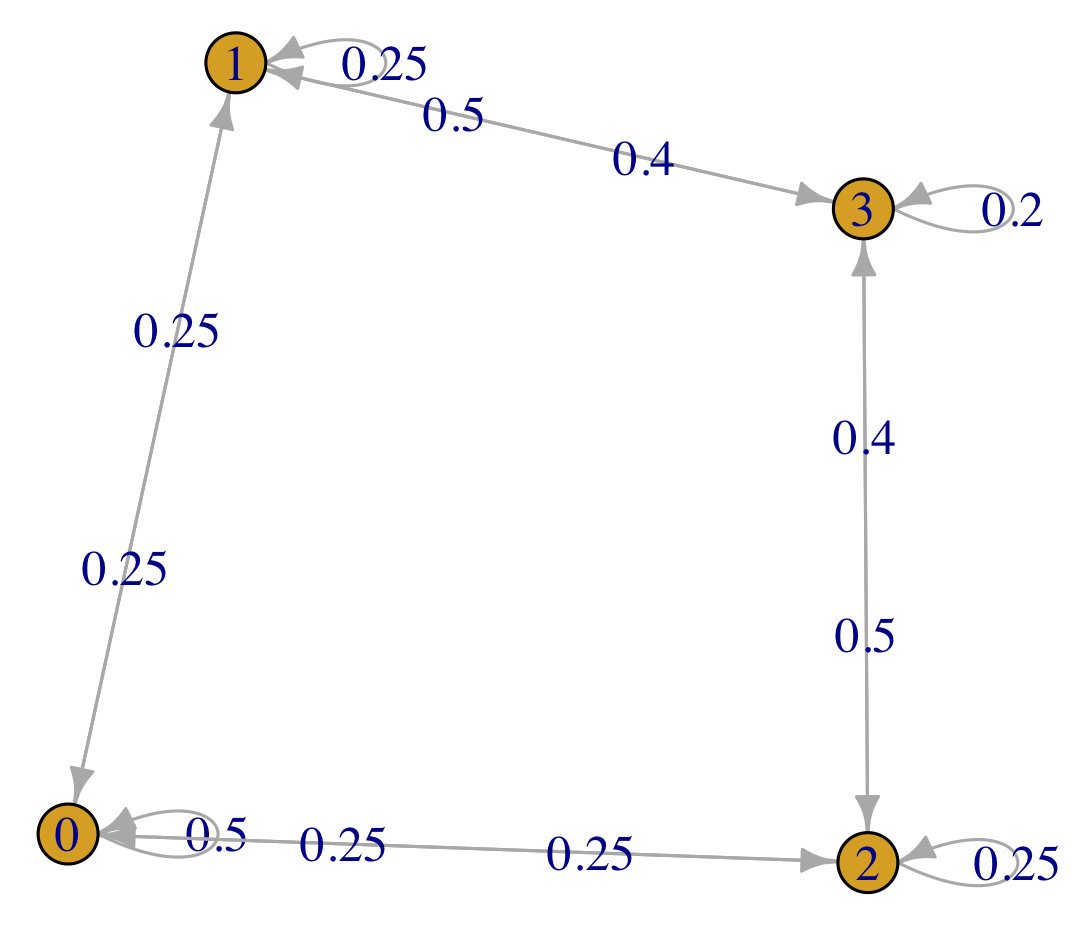
\includegraphics[scale=0.9]{gambar/contoh_dtmc_plot.png}
\end{frame}

\begin{frame}[fragile]{Simulasi DTMC di R}
    Untuk melakukan simulasi, tentukan waktu berjalannya simulasi,

\begin{minted}{r}
mc1_t <- 10    
\end{minted}

    kemudian lakukan \verb|set.seed| dengan bilangan bulat apapun, untuk keperluan \textit{reproducibility} (agar hasil selalu sama walaupun \textit{random}), misalnya 123:

\begin{minted}{r}
set.seed(123)
\end{minted}

    Barulah lakukan simulasi dengan fungsi \verb|rmarkovchain|, misalnya dengan \textit{state} awal "0"

\begin{minted}{r}
mc1_sim <- rmarkovchain(n = mc1_t, object = mc1_obj,
                        t0 = "0")
\end{minted}

Untuk \textit{random seed} yang dipilih yaitu 123, hasil simulasi yang tersimpan di \verb|mc1_sim| adalah 10 \textit{state} berikut, secara berturut-turut:

\verb|"0" "2" "3" "3" "3" "1" "0" "2" "0" "0"|

\end{frame}

\begin{frame}[fragile]{Plot Hasil Simulasi DTMC di R}
    Dengan sedikit kode, kita dapat membuat \textit{plot} hasil simulasi tersebut (ditampilkan di \textit{slide} selanjutnya).

\begin{minted}{r}
mc1_sim_factors <- factor(mc1_sim, levels = mc1_states)
mc1_sim_int <- as.integer(mc1_sim_factors)
mc1_sim_times <- 1 : mc1_t
plot(x = mc1_sim_times,
     y = mc1_sim_int,
     xlab = "Waktu (diskrit)",
     ylab = "State",
     main = "Simulasi DTMC",
     xaxt = "n", yaxt = "n")
axis(1, at = mc1_sim_times)
axis(2, at = 1 : length(mc1_states),
        labels = mc1_states)
\end{minted}
\end{frame}

\begin{frame}{Plot Hasil Simulasi DTMC di R}
    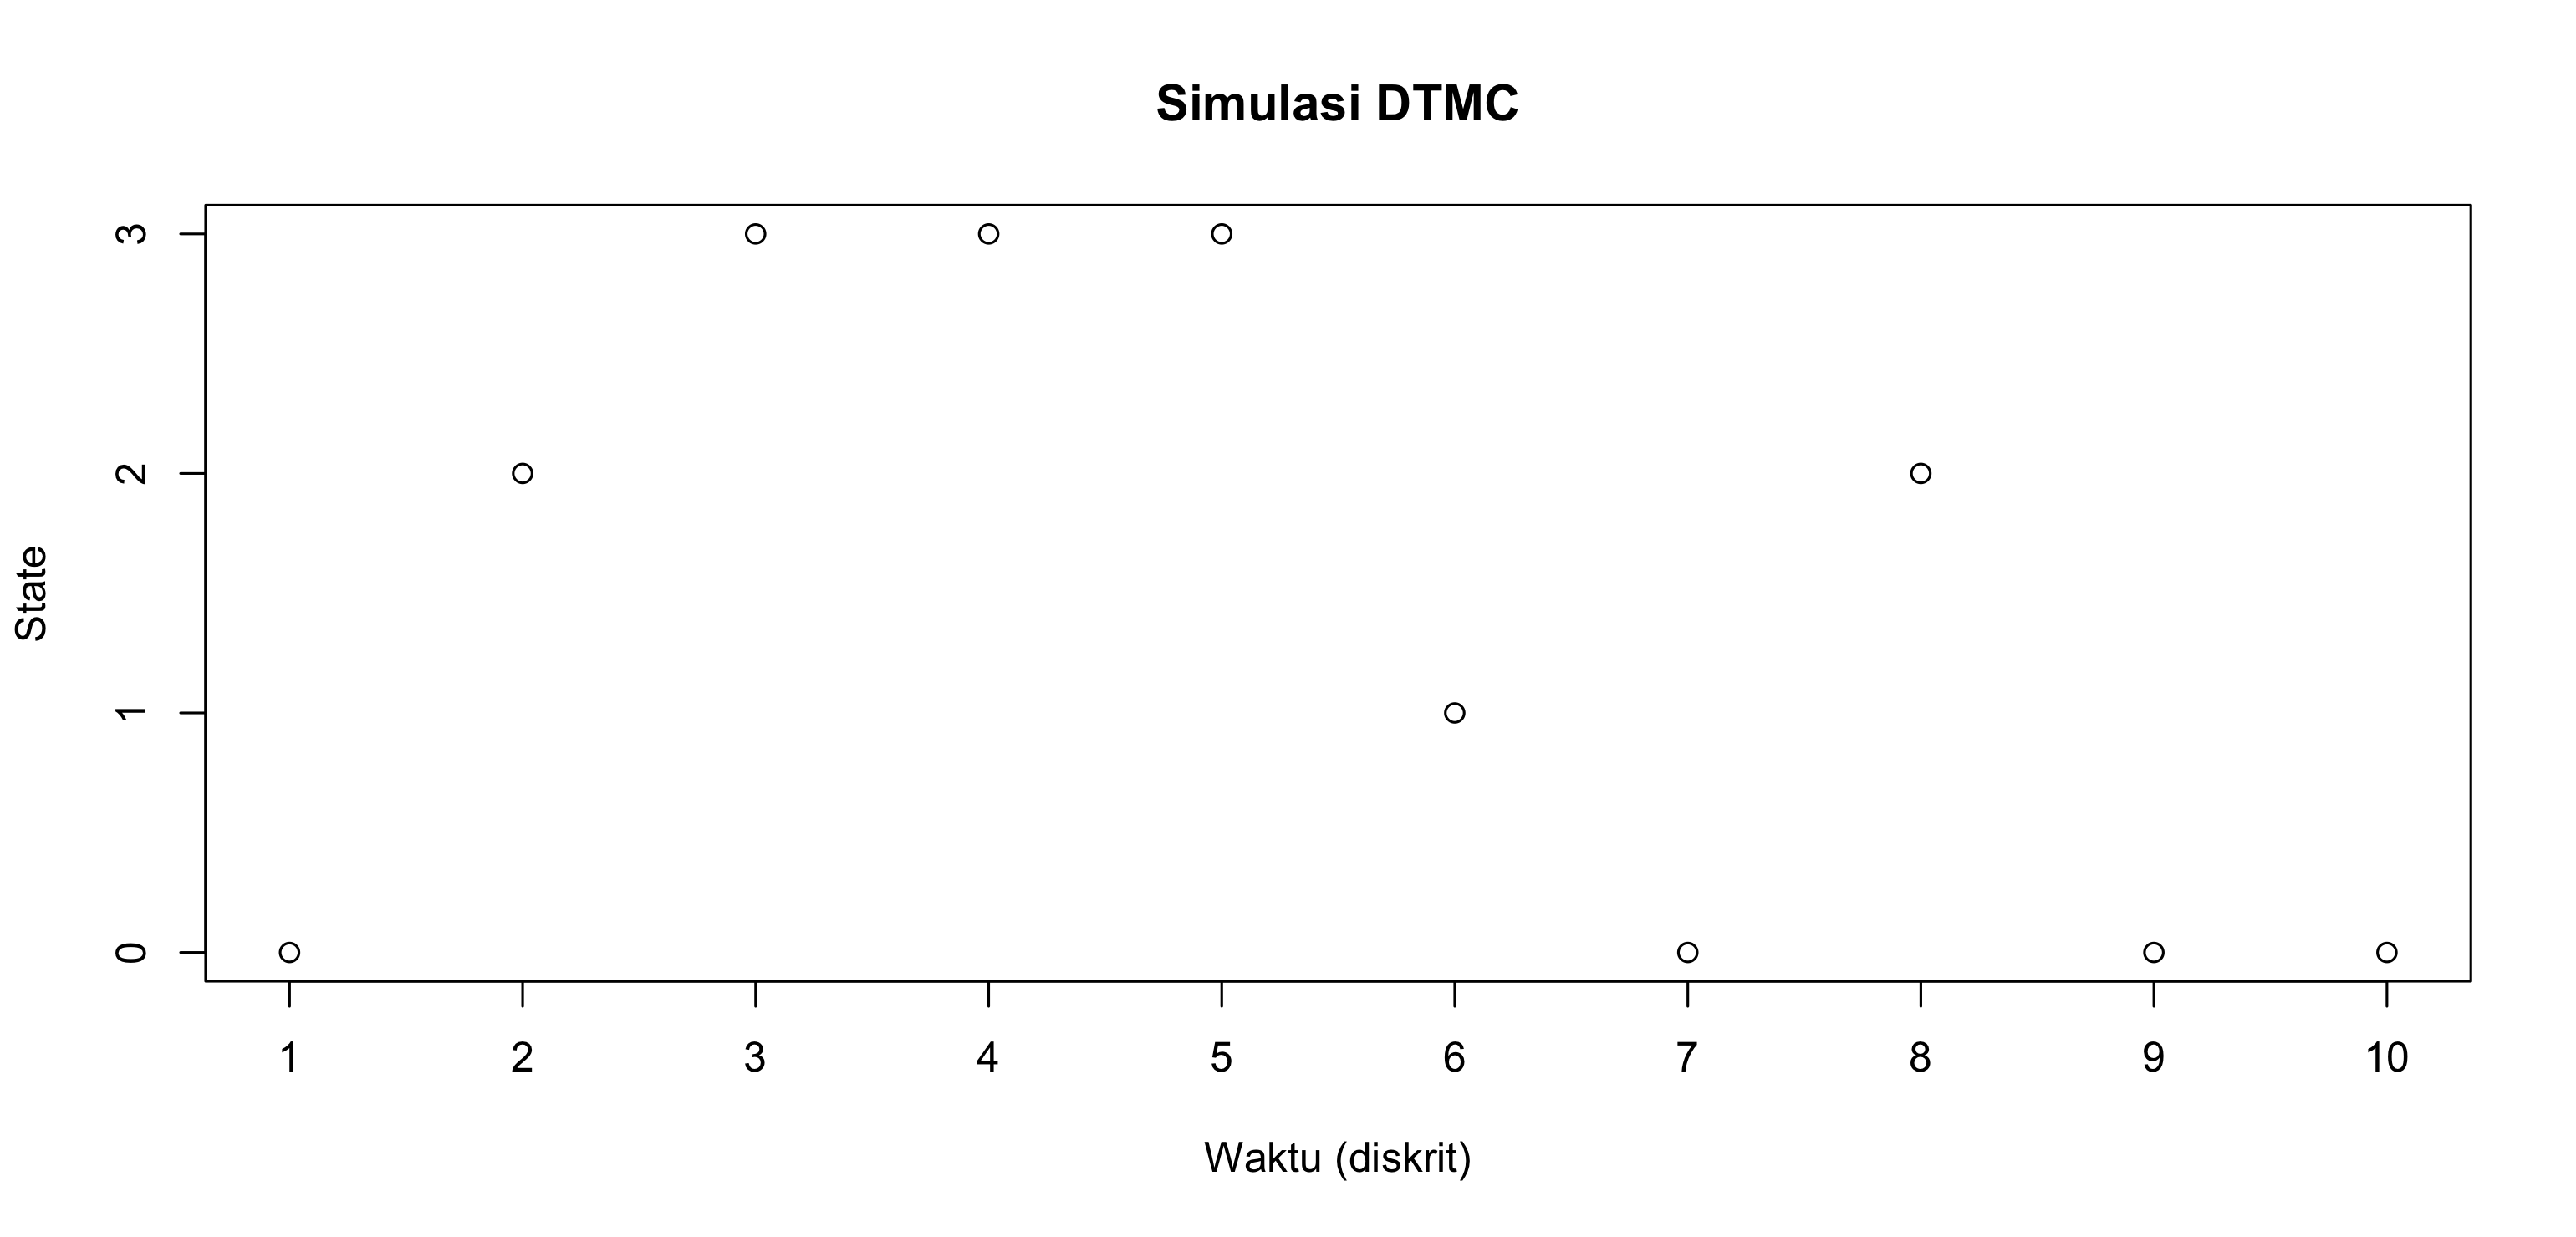
\includegraphics[scale=0.45]{gambar/contoh_dtmc_simulasi.png}
\end{frame}

\begin{frame}[fragile]{Probabilitas Jangka Panjang DTMC di R}
    Walaupun berupa proses \textit{random}, model stokastik memiliki konsep "probabilitas jangka panjang" \textit{(long-run probability)}, yaitu hitungan probabilitas secara umum berada di \textit{state} tertentu. Untuk itu, distribusi stasioner \textit{(stationary distribution)}, juga disebut \textit{steady state probabilities}, bisa dihitung.

    Di R, untuk DTMC, kita bisa memperoleh \textit{steady state probabilities} dengan

\begin{minted}{r}
steadyStates(mc1_obj)
\end{minted}

    Untuk contoh DTMC yang dibahas, hasilnya adalah

\begin{verbatim}
0         1         2         3
0.2352941 0.2352941 0.2352941 0.2941176
\end{verbatim}
    yang bisa ditulis \(p_n\) untuk \textit{steady state probability} untuk \textit{state} \(n\).
    \begin{align*}
        p_0 &\approx 0.2352941, & p_2 &\approx 0.2352941, \\
        p_1 &\approx 0.2352941, & p_3 &\approx 0.2941176
    \end{align*}
    \textbf{Catatan:} hasil bisa tergantung \textit{state} awal.
\end{frame}

\begin{frame}[fragile]{Analisis DTMC di R}
    Selain \textit{steady state probabilities}, beberapa hasil lainnya tentang DTMC juga bisa diperoleh di R, dengan fungsi \verb|summary|

\begin{minted}{r}
summary(mc1_obj)    
\end{minted}

    Hasilnya mengandung beberapa unsur DTMC yang tidak akan kita bahas di sini:

\begin{verbatim}
Unnamed Markov chain  Markov chain that is composed by: 
Closed classes: 
0 1 2 3 
Recurrent classes: 
{0,1,2,3}
Transient classes: 
NONE 
The Markov chain is irreducible 
The absorbing states are: NONE
\end{verbatim}
\end{frame}

\begin{frame}{Iklan: Kuliah Model Stokastik 1}
Di sini, kita membahas DTMC hanya sebagai pengantar untuk konsep-konsep model stokastik lainnya yang pada akhirnya berujung ke teori antrian, seperti diagram transisi. Apabila tertarik untuk mempelajari lebih lanjut, seperti tentang
\begin{itemize}
    \item pemodelan untuk berbagai persoalan menggunakan DTMC hingga penyelesaiannya,
    \item jenis-jenis \textit{state} seperti \textit{recurrent state}, \textit{transient state}, dan \textit{absorbing state}, serta
    \item sifat-sifat rantai Markov, seperti \textit{irreducible} dan periodik,
\end{itemize}
itu semua dipelajari di kuliah Model Stokastik 1 (3 SKS) yang bisa diambil semester depan (\textit{request} saja), saat ini merupakan mata kuliah wajib di semester genap (tepatnya semester 4) untuk program studi S1 Statistika dan program studi S1 Ilmu Aktuaria.

Sementara ini, kita akan lanjut membahas model stokastik yang lebih berkaitan dengan teori antrian, seperti proses Poisson.
\end{frame}

\subsection{Proses Poisson}

\begin{frame}{Distribusi Poisson}
    \begin{itemize}
        \item Proses Poisson didasari oleh distribusi Poisson, yang akan kita bahas terlebih dahulu
        \item Distribusi Poisson adalah distribusi diskrit yang memodelkan probabilitas untuk banyaknya kemunculan dalam suatu satuan waktu
        \item Hanya memliki satu parameter: rata-rata kemunculan per satuan waktu, biasa disebut \textit{rate} dan ditulis \( \lambda \), dengan syarat \( \lambda > 0 \)
        \item Contoh: \( \text{Pois}(3) \), yaitu distribusi Poisson dengan \textit{rate} \( \lambda = 3 \)

        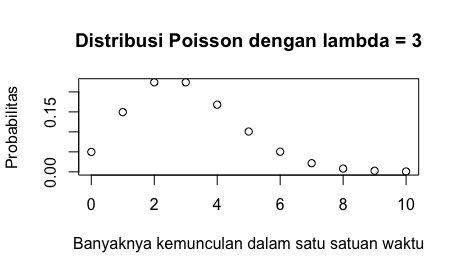
\includegraphics[scale=0.45]{gambar/dist_pois_lambda3.png}
    \end{itemize}
\end{frame}

\begin{frame}{PMF untuk Distribusi Poisson}
    %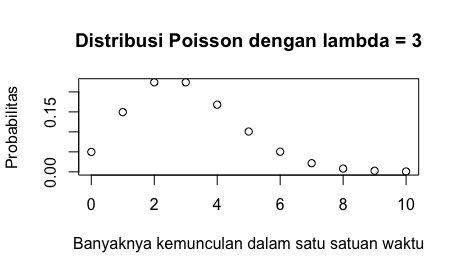
\includegraphics[scale=0.4]{gambar/dist_pois_lambda3.png}

    Misalkan variabel acak \(X\) berdistribusi Poisson dengan \textit{rate} \(\lambda\), atau biasa ditulis
    \[ X \sim \text{Pois}(\lambda) \]
    Gambar di atas adalah contoh gambar PMF \textit{(probability mass function)} dari distribusi Poisson, yaitu nilai probabilitas untuk tepat \(k\) kemunculan dalam satu satuan waktu:
    \[ \text{Pr}(X=k) = \frac{e^{-\lambda} \lambda^k}{k!} \]
    Contohnya, nilai PMF di \(k=2\) untuk \(\lambda = 3\) orang/menit adalah
    \[ \text{Pr}(X=2) = \frac{e^{-3} 3^2}{2!} \approx 0.2240418 \]
    yaitu probabilitas datangnya \textbf{tepat dua} orang dalam satu menit, jika rata-rata kedatangan adalah \(\lambda = 3\) orang/menit.
\end{frame}

\begin{frame}{CDF untuk Distribusi Poisson}
    Sebagaimana distribusi diskrit pada umumnya, CDF \textit{(cumulative distribution function)} untuk distribusi Poisson adalah sumasi PMF hingga nilai \(k\) yang ditentukan, ditulis \(\text{Pr}(X \le k)\)
    \[ \text{Pr}(X \le k) = \sum_{j=0}^{k} \text{Pr}(X = j) = \sum_{j=0}^{k} \frac{e^{-\lambda} \lambda^j}{j!} = \frac{e^{-\lambda} \lambda^0}{0!} + \dots + \frac{e^{-\lambda} \lambda^k}{k!} \]
    Interpretasinya di sini adalah probabilitas kemunculan \textbf{paling banyak} \(k\) dalam suatu satuan waktu.

    Contohnya, nilai CDF di \(k = 2\) untuk \( \lambda = 3 \) orang/menit adalah
    \begin{align*}
        \text{Pr}(X \le 2) &= \sum_{j=0}^{2} \frac{e^{-3} 3^j}{j!} = \frac{e^{-3} 3^0}{0!} + \frac{e^{-3} 3^1}{1!} + \frac{e^{-3} 3^2}{2!} \\
        &\approx 0.04978707 + 0.1493612 + 0.2240418 \\
        &\approx 0.4231901
    \end{align*}
    yaitu probabilitas datangnya \textbf{paling banyak dua} orang dalam satu menit, jika rata-rata kedatangan adalah \(\lambda = 3\) orang/menit.
\end{frame}

\begin{frame}[fragile]{PDF dan CDF Poisson di R}
    Untuk distribusi Poisson, R menyediakan fungsi \verb|dpois| untuk PMF dan \verb|ppois| untuk CDF. Misalnya, kita bisa menghitung \( \text{Pr}(X=2) \) dengan
\begin{minted}{r}
dpois(2, lambda = 3)
\end{minted}
    Hasil: \verb|0.2240418|

    Kita bisa menghitung \( \text{Pr}(X \le 2) \) dengan
\begin{minted}{r}
ppois(2, lambda = 3)
\end{minted}
    Hasil: \verb|0.4231901|

    atau bisa juga secara "manual" sebagai sumasi PMF, dan diperoleh hasil yang sama:
\begin{minted}{r}
dpois(0, lambda = 3) +
  dpois(1, lambda = 3) +
  dpois(2, lambda = 3)
\end{minted}
\end{frame}

\begin{frame}[fragile]{Plot Distribusi Poisson di R}
    Plot PMF \(\text{Pois}(3)\) di beberapa \textit{slide} sebelumnya diperoleh dengan kode R berikut. Intinya, kita memang menghitung nilai PMF Poisson di \(0, \dots, 10\), kemudian menampilkannya.

\begin{minted}[fontsize=\small]{r}
par_lambda <- 3
x_pois <- 0 : 10
p_pois <- dpois(x_pois, lambda = par_lambda)
plot(x_pois, p_pois,
     main = "Distribusi Poisson dengan lambda = 3",
     xlab = "Banyaknya kemunculan dalam satu satuan waktu",
     ylab = "Probabilitas")
\end{minted}

    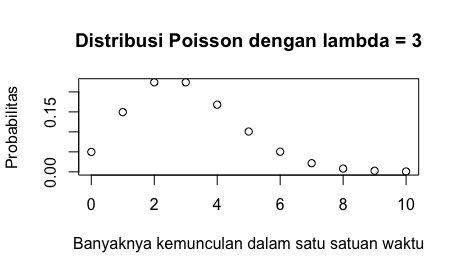
\includegraphics[scale=0.4]{gambar/dist_pois_lambda3.png}
\end{frame}

\begin{frame}{Sifat-Sifat Distribusi Poisson}
    Untuk variabel acak \(X \sim \text{Pois}(\mu)\), berlaku
    \begin{itemize}
        \item \(\text{E}\brackets{X} = \mu\), yaitu ekspektasi atau rata-rata untuk \(X\) adalah \(\mu\)
        \item \(\text{Var}\brackets{X} = \mu\), yaitu variansi untuk \(X\) juga \(\mu\)
    \end{itemize}
    sehingga \(\text{E}\brackets{X} = \text{Var}\brackets{X} = \mu\).

    Oleh karena itu, distribusi Poisson \(\text{Pois}(\lambda)\) terkadang disebut "memiliki parameter \(\lambda\)", "memiliki \textit{rate} \(\lambda\)", atau "memiliki rata-rata \(\lambda\)", artinya sama.

    Selain itu, hasil jumlah dua variabel acak independen yang berdistribusi Poisson juga berdistribusi Poisson dengan \textit{rate} berupa hasil jumlah dari kedua \textit{rate}, atau bisa ditulis
    \[\text{Pois}(\mu) + \text{Pois}(v) \sim \text{Pois}(\mu + v)\]
    %selama \(\text{Pois}(\mu)\) dan \(\text{Pois}(v)\) independen, karena

    Penggunaan distribusi Poisson untuk memodelkan kemunculan dirumuskan sebagai model stokastik bernama proses Poisson, dibahas setelah ini.
\end{frame}

\begin{frame}{Definisi Proses Poisson}
    Proses Poisson dengan \textit{rate} \(\lambda > 0\) adalah model stokastik bernilai bulat, misalnya dinotasikan \( \braces{X(t); \, t \ge 0} \) dengan \(X(t)\) melambangkan banyaknya kemunculan dari waktu nol sampai \(t\), yang memenuhi
    \begin{itemize}
        \item \(X(0) = 0\), yaitu belum ada kemunculan di waktu \(t=0\);
        \item \textit{independent increments}, yaitu variabel-variabel acak berikut (masing-masing berupa selisih kemunculan, yaitu banyaknya kemunculan dalam interval waktu)
        \[ X\pars{t_i} - X\pars{t_{i-1}}, \quad 0 \le t_1 < t_2 < \dots < t_n \]
        semuanya saling independen; dan
        \item untuk tiap titik waktu \(s \ge 0\) dan durasi \(t > 0\), berlaku
        \[X(s+t) - X(s) \sim \text{Pois}(\lambda t)\]
        yaitu banyaknya kemunculan dalam interval waktu \(\brackets{s,s+t}\) berdistribusi \(\text{Pois}(\lambda t)\)
    \end{itemize}
\end{frame}

\begin{frame}{Sifat-Sifat Proses Poisson}
    Jelas bahwa \(\text{E}\brackets{X(t)} = \text{Var}\brackets{X(t)} = \lambda t\) karena
    \[X(t) = X(0+t) - X(0) \sim \text{Pois}(\lambda t)\]
    Selain itu, untuk tiap titik waktu \(s \ge 0\) dan durasi \(t > 0\), berlaku
    \[\text{Pr}\brackets{X(s+t) - X(s) = k} = \frac{e^{-\lambda t}\pars{\lambda t}^k}{k!}\]
    sesuai rumus PMF Poisson, tepatnya \(\text{Pois}(\lambda t)\). Maka,
    \[\text{Pr}\brackets{X(t) = k} = \text{Pr}\brackets{X(0+t) - X(0) = k} = \frac{e^{-\lambda t}\pars{\lambda t}^k}{k!}\]
    sehingga bisa disimpulkan
    \[\text{Pr}\brackets{X(s+t) - X(s) = k} = \text{Pr}\brackets{X(t) = k} = \frac{e^{-\lambda t}\pars{\lambda t}^k}{k!}\]
\end{frame}

\begin{frame}{\textit{Stationary increments} dalam proses Poisson}
    Untuk proses Poisson \(\braces{X(t)}\), sudah ditunjukkan bahwa
    \[\text{Pr}\brackets{X(s+t) - X(s) = k} = \text{Pr}\brackets{X(t) = k}\]
    Pilih \(b = s+t\) dan \(a = s\) agar \(t = b-s = b-a\), sehingga
    \[\text{Pr}\brackets{X(b) - X(a) = k} = \text{Pr}\brackets{X\pars{b-a} = k}\]
    Kedua persamaan di atas adalah sifat yang sama, yang disebut \textit{stationary increments}.
    %\textbf{Kesamaan probabilitas mengindikasikan kesamaan PMF, yang mengimplikasikan kesamaan distribusi.}
\end{frame}

\begin{frame}{\textit{Interarrival times} dan \textit{waiting/arrival times}}
    Sejauh ini, kita berurusan dengan banyaknya kemunculan dalam interval waktu.
    
    Kita juga bisa membalikkannya, agar berurusan dengan lama waktu antar kemunculan, juga disebut waktu antar kedatangan \textit{(interarrival time)} atau \textit{sojourn time}, biasa dilambangkan \( T_n \) untuk durasi antara kemunculan ke-\((n-1)\) dengan kemunculan ke-\(n\). Karena kemunculan di sini bersifat acak, \textit{interarrival time} \(T_n\) juga berupa variabel acak, dan \(\braces{T_n, \, n=1,2,\dots}\) menjadi barisan variabel acak, disebut barisan \textit{interarrival times}, dimulai dari \(T_1\) sebagai durasi dari awal dimulainya proses Poisson hingga kemunculan pertama. Tiap \(T_i\) saling independen.

    Terkadang, kita ingin berurusan dengan lama waktu dari awal proses hingga kedatangan ke-\(n\), daripada lama waktu antar kedatangan. Untuk itu, variabel acak \textit{waiting time} atau \textit{arrival time} didefinisikan
    \[W_n = T_1 + T_2 + \dots + T_n\]
\end{frame}

\begin{frame}{\(T_1\) berdistribusi eksponensial}
    Bagaimana distribusi dari \(T_n\)? Mari kita tinjau \(T_1\) terlebih dahulu. Kita bisa tinjau CDFnya yaitu \(\text{Pr}(T_1 \le t)\), lalu kita hubungkan dengan kemunculan: kejadian \(\brackets{T_1 \le t} = \brackets{W_1 \le t}\), bahwa kemunculan pertama sudah tercapai, itu sama saja dengan kejadian \(\brackets{X(t) \ne 0}\), yaitu banyaknya kemunculan sudah tidak lagi nol. Maka probabilitas kedua kejadian sama, sehingga
    \begin{align*}
        \text{Pr}\pars{T_1 \le t} &= \text{Pr}\brackets{X(t) \ne 0}
        = 1 - \text{Pr}\brackets{X(t) = 0}
        = 1 - \frac{e^{-\lambda t}\pars{\lambda t}^0}{0!} \\
        &= 1 - \frac{e^{-\lambda t}(1)}{1}
        = 1 - e^{-\lambda t}
    \end{align*}
    yaitu CDF distribusi eksponensial (mari kita bahas!), sehingga \(T_1 \sim \text{Exp}(\lambda)\), yaitu variabel acak \(T_1\) berdistribusi eksponensial dengan parameter \(\lambda\) yang juga disebut \textit{rate}.
\end{frame}

\begin{frame}{Distribusi Eksponensial}
    Distribusi eksponensial adalah suatu distribusi kontinu dengan satu parameter saja, biasa ditulis \(\lambda > 0\) (kebetulan?), dan biasa disebut \textit{rate} (kebetulan?). Apabila dimisalkan
    \[T \sim \text{Exp}(\lambda)\]
    yaitu \(T\) berdistribusi eksponensial dengan \textit{rate} \(\lambda\), bisa ditulis fungsi PDF \textit{(probability density function)}
    \[f_T(t) = \begin{cases}
        \lambda e^{-\lambda t}, & t \ge 0 \\
        0, & t < 0
    \end{cases}\]
    dan CDF berikut (dihitung sebagai integral dari \(-\infty\) sampai \(t\) dari PDF, sebagaimana distribusi kontinu pada umumnya)
    \[F_T(t) = \text{Pr}(T \le t) = \begin{cases}
        1 - e^{-\lambda t}, & t \ge 0 \\
        0, & t < 0
    \end{cases}\]
\end{frame}

\begin{frame}{Sifat-Sifat Distribusi Eksponensial}
    Untuk variabel acak \(T \sim \text{Exp}(\lambda)\), berlaku
    \[\text{E}\brackets{T} = \frac{1}{\lambda}, \quad \text{Var}\brackets{T} = \frac{1}{\lambda^2}\]
    sehingga \(\text{Var}\brackets{T} = \text{E}\brackets{T}^2\).

    Daripada menulis CDF eksponensial yaitu \(\text{Pr}(T \le t) = 1 - e^{-\lambda t}\), lazim ditulis
    \[\text{Pr}(T > t) = e^{-\lambda t}\]
    sehingga kita bisa membuktikan bahwa variabel acak \(T\) berdistribusi eksponensial melalui pembuktian persamaan di atas daripada langsung membuktikan bentuk CDFnya. \\[0.25em]

    Selain itu, apabila variabel-variabel acak \(T_1, \dots, T_n\) saling independen dan \(T_i \sim \text{Exp}(\lambda_i)\) untuk tiap \(i=1,\dots,n\), maka
    \[\text{min}\braces{T_1, \dots, T_n} \sim \text{Exp}\pars{\lambda_1 + \dots + \lambda_n}\]
\end{frame}

\begin{frame}{Sifat \textit{Memoryless} dan Distribusi Eksponensial}
    Yang terpenting, distribusi eksponensial memenuhi \textit{memoryless property} sebagai berikut:
    \[\text{Pr}\pars{T > t+s \; \middle| \; T > s} = \text{Pr}\pars{T > t}\]
    untuk sembarang titik waktu \(s \ge 0\) dan durasi \(t > 0\), karena
    \begin{align*}
        \text{Pr}\pars{T > t+s \; \middle| \; T > s} &= \frac{\text{Pr}\pars{T>t+s, T>s}}{\text{Pr}\pars{T>s}} = \frac{\text{Pr}\pars{T>t+s}}{\text{Pr}\pars{T>s}} \\
        &= \frac{e^{-\lambda \pars{t+s}}}{e^{-\lambda s}} = e^{-\lambda t} = \text{Pr}\pars{T > t}
    \end{align*}
    Bahkan, bisa dibuktikan (tidak dibahas di sini) bahwa distribusi eksponensial adalah \textbf{satu-satunya distribusi kontinu yang memenuhi \textit{memoryless property}}. Artinya, apabila \(T\) adalah variabel acak kontinu yang memenuhi \textit{memoryless property}, haruslah \(T \sim \text{Exp}(\lambda)\) untuk suatu \(\lambda > 0\).
\end{frame}

% (cara salah, batal)
%\begin{frame}{\(T_n\) berdistribusi eksponensial}
    %Dengan cara yang serupa seperti \(T_1\), mari kita tinjau distribusi \(T_n\). Kejadian \(\brackets{T_n \le t}\), bahwa kemunculan ke-\(n\) sudah tercapai, sama dengan kejadian \(\brackets{X(t) \ge n}\), yaitu banyaknya kemunculan hingga titik waktu \(t\) setidaknya sebanyak \(n\), sehingga
    %\begin{align*}
        %\text{Pr}\pars{T_n \le t} &= \text{Pr}\brackets{X(t) \ge n} = 1 - \text{Pr}\brackets{X(t) < n} \\
        %&= 1 - \sum_{j=0}^{n-1} \text{Pr}\brackets{X(t) = j} = 1 - \sum_{j=0}^{n-1} \frac{e^{-\lambda t}\pars{\lambda t}^j}{j!}
    %\end{align*}
    %Mengingat bahwa jumlahan distribusi Poisson yang saling independen juga berdistribusi Poisson dengan \textit{rate} yang dijumlah,
    %\[\text{Pr}\pars{T_n \le t} = 1 - \sum_{j=0}^{n-1} \frac{e^{-\lambda t}\pars{\lambda t}^j}{j!} = 1 - \frac{e^{-n\lambda t}\pars{n\lambda t}^j}{j!}\]
%\end{frame}
% (salah juga)
%\begin{frame}{\(T_n\) berdistribusi eksponensial}
    %Sekarang, mari kita tinjau distribusi \(T_n\). Perhatikan bahwa \(T_n = W_n - W_{n-1}\), sehingga berdasarkan \textit{memoryless property} dari distribusi \(T \sim \text{Exp}(\lambda)\),
    %\begin{align*}
        %\text{Pr}\brackets{T > W_{n-1} + T_n \; \middle| \; T > T_n} = \text{Pr}\pars{T > W_{n-1}}
    %\end{align*}
%\end{frame}
% (gagal lagi, au ah)
%\begin{frame}{\(T_n\) berdistribusi eksponensial}
    %Dengan cara yang mirip seperti \(T_1\), mari kita tinjau distribusi \(T_n\). Namun, daripada meninjau CDF yaitu \(\text{Pr}\pars{T_n \le t}\), kita tinjau \(\text{Pr}\pars{T_n > t}\).
    %Kejadian \(\brackets{T_n > t}\), bahwa kemunculan ke-\(n\) belum tercapai, sama dengan kejadian \(\brackets{X(t) < n}\), yaitu banyaknya kemunculan hingga titik waktu \(t\) masih kurang dari \(n\). Sehingga, %Perhatikan bahwa \(T_n = W_n - W_{n-1}\).
    %\begin{align*}
        %\text{Pr}\pars{T_n \le t} &= \text{Pr}\brackets{X(t) < n} = \text{Pr}\brackets{X\pars{t - W_{n-1} + W_{n-1}} < n}
    %\end{align*}
    %Berdasarkan sifat proses Poisson,
    %\begin{align*}
        %\text{Pr}\brackets{X\pars{t - W_{n-1} + W_{n-1}} - X\pars{W_{n-1}} < n} = \text{Pr}\brackets{X\pars{t - W_{n-1}} < n}
    %\end{align*}
%\end{frame}
% menggeser meragukan...
%\begin{frame}{\(T_n\) berdistribusi eksponensial}
    %Dengan cara yang mirip seperti \(T_1\), mari kita tinjau distribusi \(T_n\). Namun, daripada meninjau CDF yaitu \(\text{Pr}\pars{T_n \le t}\), kita tinjau \(\text{Pr}\pars{T_n > t}\). Kejadian \(\brackets{T_n > t}\), bahwa kemunculan ke-\(n\) belum tercapai, sama dengan kejadian \(\brackets{X(t) < n}\), yaitu banyaknya kemunculan hingga titik waktu \(t\) masih kurang dari \(n\). Sehingga,
    %\begin{align*}
        %\text{Pr}\pars{T_n > t} &= \text{Pr}\brackets{X(t) < n} = \text{Pr}\brackets{X(t) - (n-1) < n - (n-1)} \\
        %&= \text{Pr}\brackets{X(t) - X\pars{W_{n-1}} < 1} = \text{Pr}\brackets{X(t) - X\pars{W_{n-1}} = 0} \\
        %%&= \text{Pr}\brackets{X\pars{t - W_{n-1} + W_{n-1}} - X\pars{W_{n-1}} = 0} \\
        %&\text{Berdasarkan sifat \textit{stationary increments},} \\
        %&= \text{Pr}\brackets{X\pars{t - W_{n-1}} = 0} \\
        %&\text{"Menggeser" proses Poisson ke kemunculan ke-}(n-1), \\
        %&= \text{Pr}\brackets{X(t) = 0} = \frac{e^{-\lambda t}\pars{\lambda t}^0}{0!} = e^{-\lambda t}
    %\end{align*}
    %Dengan demikian, \(T_n \sim \text{Exp}(\lambda)\).
%\end{frame}
% ALL THIS TIME I BEGAN WITH T_n > t AND THOUGHT IT MEANT THE WAITING TIME IS MORE THAN t........ YET SOMEHOW I KNEW, FOR ALL STEPS AFTER THAT, THAT T_n IS INTERARRIVAL... NO WONDER I KEEP GETTING IT WRONG THE WHOLE DAY DAMN IT!
%\begin{frame}{\(T_n\) berdistribusi eksponensial}
    %Dengan cara yang mirip seperti \(T_1\), mari kita tinjau distribusi \(T_n\) melalui CDF.
    %%Namun, daripada meninjau CDF yaitu \(\text{Pr}\pars{T_n \le t}\), kita tinjau \(\text{Pr}\pars{T_n > t}\). Kejadian \(\brackets{T_n > t}\), bahwa kemunculan ke-\(n\) belum tercapai, sama dengan kejadian \(\brackets{X(t) < n}\), yaitu banyaknya kemunculan hingga titik waktu \(t\) masih kurang dari \(n\).
    %Kejadian \(\brackets{T_n \le t}\), bahwa kemunculan ke-\(n\) sudah tercapai, sama dengan kejadian \(\brackets{X(t) \ge n}\), yaitu banyaknya kemunculan hingga titik waktu \(t\) setidaknya sudah sebanyak \(n\).
    %%Lebih tepatnya, untuk mempermudah, kita misalkan \(T_{n-1} = s\) sehingga \(0 < s < t\), yaitu 
    %Dengan demikian, \(T_n \sim \text{Exp}(\lambda)\).
%\end{frame}
% let's get it right this time
\begin{frame}{\(T_n\) berdistribusi eksponensial}
    Mari kita tinjau distribusi \(T_n\). Karena distribusi \(T_1\) sudah diketahui, kita bisa mencoba pendekatan perbandingan. Kita juga bisa meninjau probabilitas \(\brackets{T_2 > t}\) daripada CDF \(\brackets{T_2 \le t}\).
    
    Misalkan \(s > 0\) dan \(t > 0\) adalah dua durasi, misalnya untuk dua kemunculan berturut-turut. Perhatikan bahwa \( (0,s] \) dan \( (s, s+t] \) adalah dua interval yang saling lepas karena \( 0 < s < s+t \), sehingga berdasarkan sifat \textit{independent increments}, variabel acak \(X\pars{s+t} - X\pars{s}\) dan \(X\pars{s} - X\pars{0} = X\pars{s}\) saling bebas; 
    %Sehingga, apabila kita hitung probabilitas bersyarat seperti berikut, syarat akan hilang:
    apabila dihitung probabilitas bersyarat seperti berikut, syarat hilang:
    \begin{align*}
        \text{Pr}\pars{T_2 > t \; \middle| \; T_1 = s} &= \text{Pr}\brackets{X\pars{s+t} - X\pars{s} = 0 \; \middle| \; X\pars{s} = 1 } \\
        &= \text{Pr}\brackets{X\pars{s+t} - X\pars{s} = 0} \quad \pars{= \text{Pr}\pars{T_2 > t}} \\
        &\text{Berdasarkan sifat \textit{stationary increments,}} \\
        &= \text{Pr}\brackets{X\pars{t} = 0} = \frac{e^{-\lambda t} \pars{\lambda t}^0}{0!} = e^{-\lambda t}
    \end{align*}
    sehingga \(T_2 \sim \text{Exp}(\lambda)\). Dengan bukti serupa, \(T_n \sim \text{Exp}(\lambda)\).
    %Dengan bukti serupa, dapat disimpulkan \(T_n \sim \text{Exp}(\lambda)\) untuk \(n = 1, 2, 3, \dots\)
\end{frame}

\begin{frame}{Contoh Proses Poisson: Kedatangan Pelanggan}
    Kedatangan pelanggan di toko tertentu mengikuti proses Poisson dengan \textit{rate} \(\lambda = 4\) orang/jam. Toko buka pukul 09.00 pagi. Tentukan probabilitas bahwa tepat satu pelanggan telah datang ketika sudah pukul 09.30 pagi DAN tepat lima pelanggan telah datang ketika sudah pukul 11.30 siang.

    \textbf{Jawab:} misalkan \(t\) bersatuan jam (agar \(\lambda = 4\) orang/jam), dan dipasang \(t=0\) untuk pukul 09.00. Memanfaatkan \textit{independent increments} antar variabel acak \(X\pars{\frac{5}{2}} - X\pars{\frac{1}{2}}\) dengan \(X\pars{\frac{1}{2}}\),
    \begin{align*}
        \text{Pr}&\braces{X\pars{\frac{1}{2}} = 1, \, X\pars{\frac{5}{2}} = 5} \\
        &= \text{Pr}\braces{X\pars{\frac{1}{2}} = 1, \, X\pars{\frac{5}{2}} - X\pars{\frac{1}{2}} = 5-1} \\
        &= \text{Pr}\braces{X\pars{\frac{1}{2}} = 1} \text{Pr}\braces{X\pars{2} = 4} \\
        &= \braces{ \frac{e^{-4(1/2)} \pars{4(1/2)}^1}{1!} }\braces{ \frac{e^{-4(2)} \pars{4(2)}^4}{4!} }
        %= \pars{2e^{-2}} \pars{\frac{512}{3}e^{-8}}
        \approx 0.0154965
    \end{align*}
\end{frame}

\begin{frame}{Simulasi Proses Poisson}
    Simulasi proses Poisson bisa dilakukan dengan langkah-langkah berikut.
    \begin{enumerate}
        \item Tetapkan \textit{rate} \(\lambda\) dan banyaknya kemunculan \(n\) yang ingin disimulasikan, lalu hasilkan barisan \textit{interarrival times} \(\braces{T_i, \, i = 1, \dots, n}\) dengan menarik \(n\) buah data \textit{random} dari \(\text{Exp}(\lambda)\).
        \item Susun barisan \textit{arrival times} \(\braces{W_i, \, i = 1, \dots, n}\) dengan menghitung jumlahan kumulatif atau \textit{cumulative sum} sesuai definisi:
        \[W_i = T_1 + \dots + T_i\]
        \item Tampilkan \textit{plot} kemunculan ke-\(i\), \( i = 1, \dots, n \) terhadap barisan \textit{arrival times}, sebagai \textit{plot} hasil simulasi kemunculan agar bisa melihat kapan munculnya.
    \end{enumerate}
\end{frame}

\begin{frame}[fragile]{Simulasi Proses Poisson di R}
    Menetapkan \(\lambda\) dan \(n\),
\begin{minted}{r}
pp_lambda <- 4
pp_n <- 10
\end{minted}
    Menghasilkan barisan \textit{interarrival times},
\begin{minted}{r}
set.seed(2024)
pp_interarrival <- rexp(pp_n, rate = pp_lambda)
\end{minted}
    Menyusun barisan \textit{arrival times},
\begin{minted}{r}
pp_arrival <- cumsum(pp_interarrival)    
\end{minted}
    Dengan \textit{seed} 2024, data hasil simulasi yang tersimpan di \verb|pp_arrival| adalah:
\begin{verbatim}
0.1684713 0.4126256 0.5028073 0.6018938 0.8472178
1.0737138 1.0943433 1.1837221 1.3761243 1.3988369
\end{verbatim}
\end{frame}

\begin{frame}[fragile]{Plot Hasil Simulasi Proses Poisson di R}
    Dengan sedikit kode, hasil simulasi proses Poisson bisa ditampilkan sebagai \textit{plot} kemunculan ke-\(i\) terhadap barisan \textit{arrival times}. Hasil \textit{plot} ditampilkan di \textit{slide} selanjutnya. (Kemunculan ke-"nol" dengan \textit{arrival time} "nol" juga "diadakan" hanya agar titik awal proses Poisson tergambarkan.)
\begin{minted}{r}
plot(x = c(0, pp_arrival),
     y = 0 : length(pp_arrival),
     type = "s",
     xlab = "Waktu",
     ylab = "Kedatangan",
     main = "Simulasi Proses Poisson dengan lambda = 4")
\end{minted}
\end{frame}

\begin{frame}{Plot Hasil Simulasi Proses Poisson di R}
    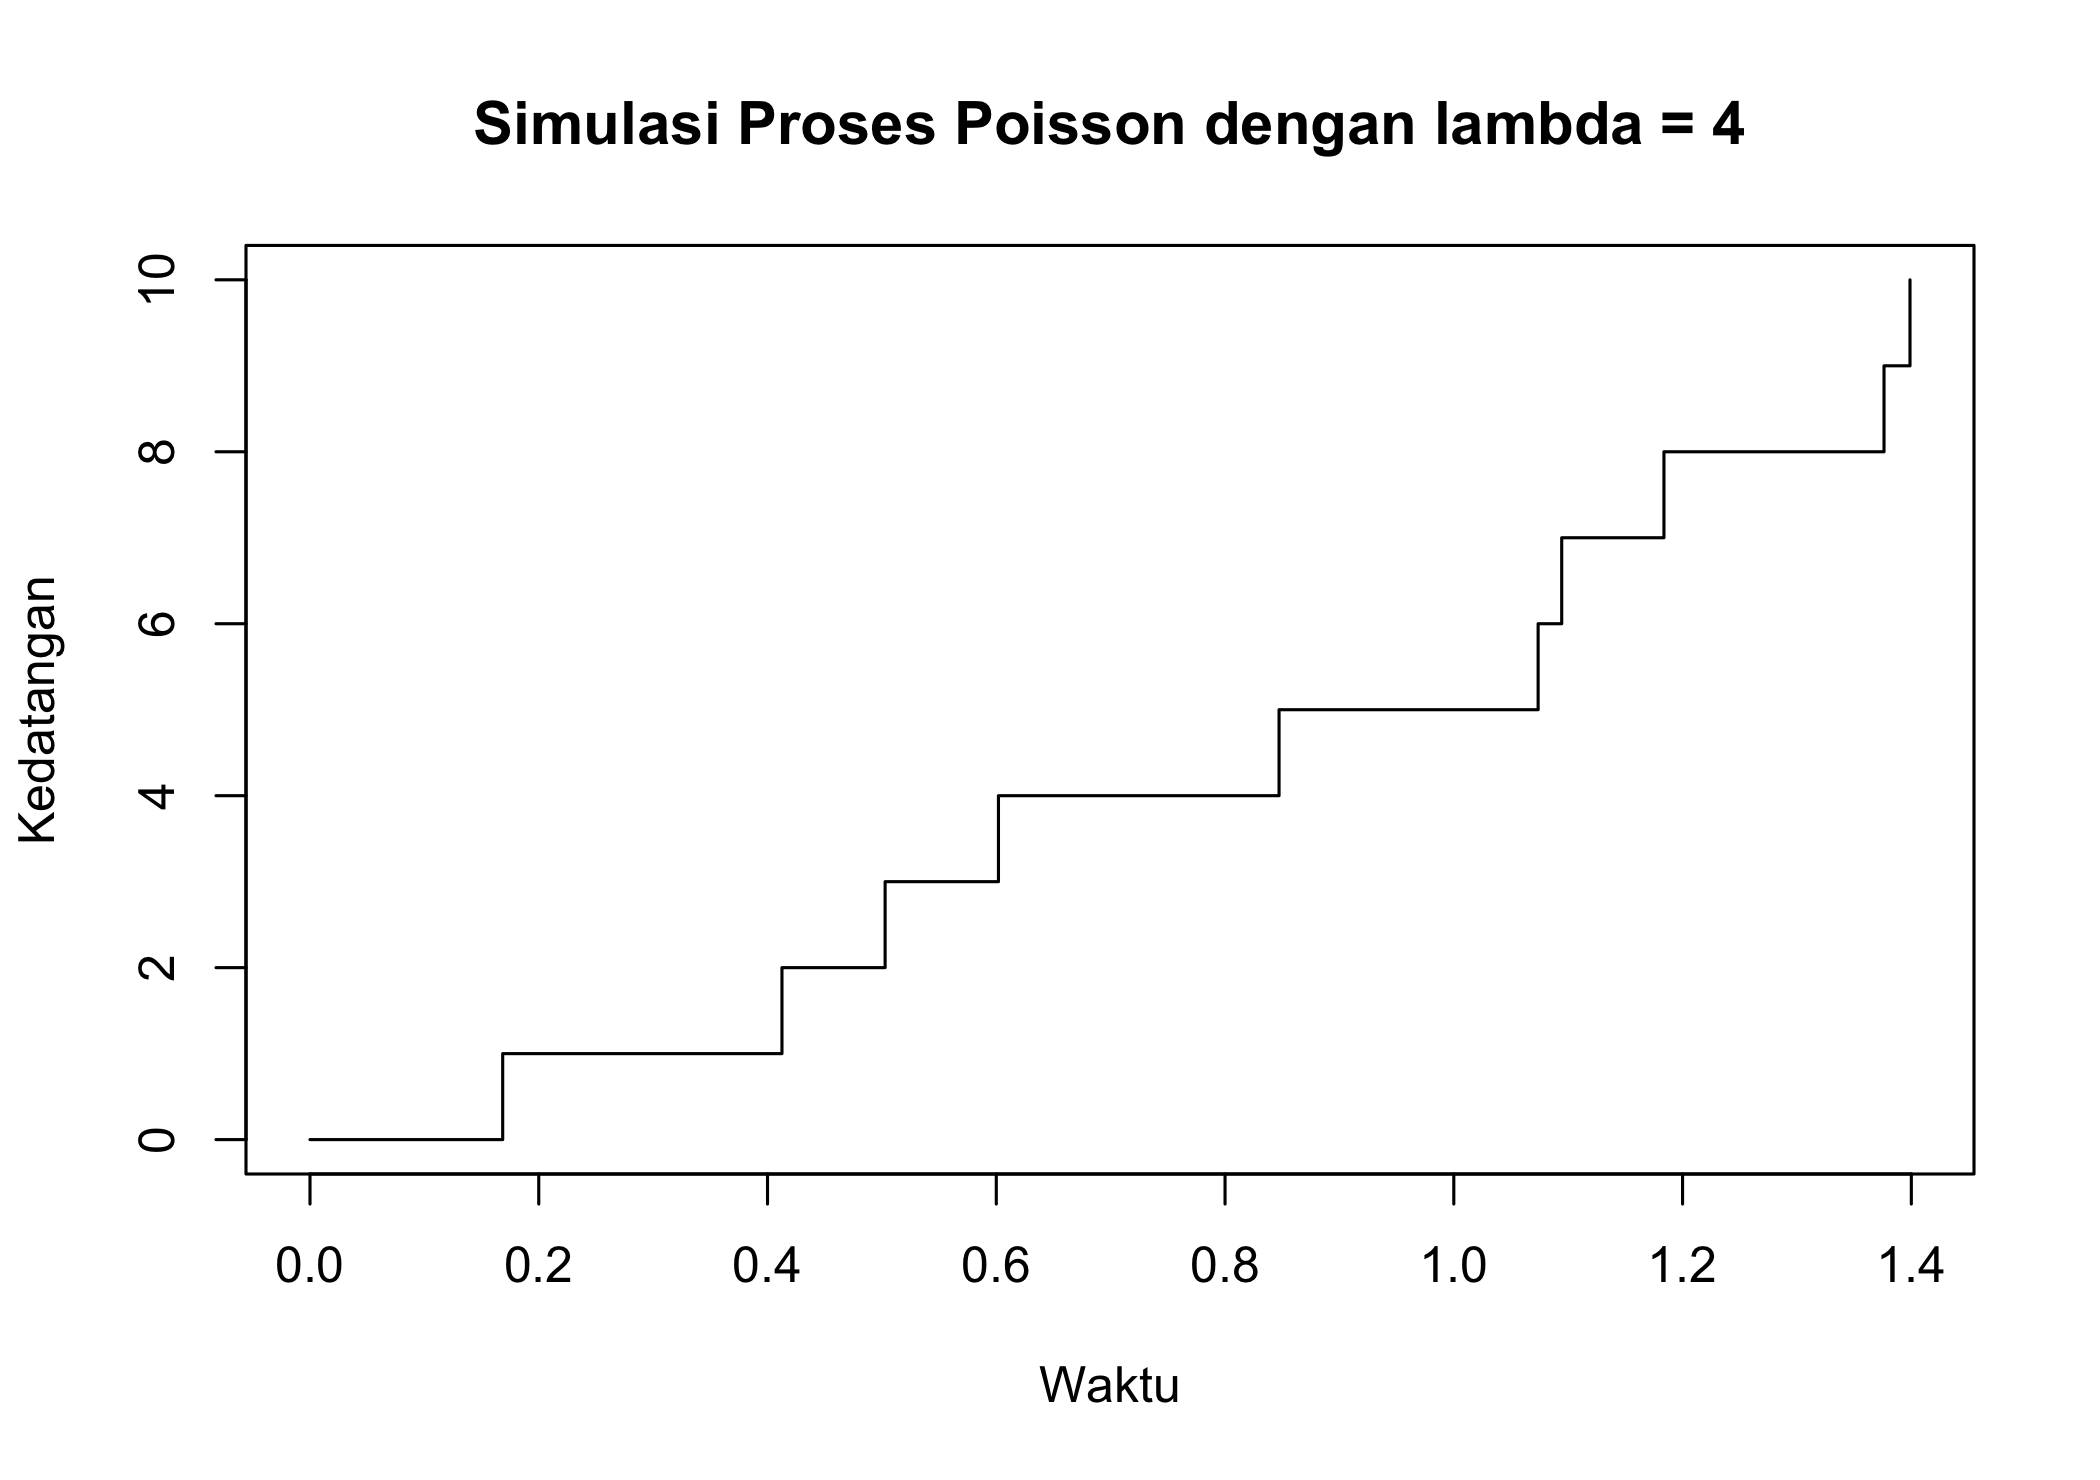
\includegraphics[scale=0.65]{gambar/proc_pois_lambda4_sim.png}
\end{frame}

\begin{frame}{Iklan (2): Kuliah Model Stokastik 1}
    Proses Poisson adalah model stokastik, sehingga juga dipelajari di kuliah Model Stokastik 1 (3 SKS) di samping DTMC. Selain dasar teori yang lebih mendalam, seperti mempelajari konsep \textit{counting process} yang mendasarinya atau bahkan notasi \textit{little-o}, berbagai contoh pemodelan dan aplikasi proses Poisson juga dibahas di sana, sedangkan di sini hanya dibahas sebagian tentang proses Poisson untuk menunjang perkuliahan tentang teori antrian. Apabila tertarik mempelajari lebih lanjut, silakan ambil kuliah Model Stokastik 1 semester depan. \\[0.5em]
    
    Bagaimanapun juga, proses Poisson sebenarnya adalah kasus khusus dari CTMC, yang selanjutnya kita bahas.
\end{frame}

\subsection{Rantai Markov Waktu Kontinu (CTMC)}

\begin{frame}{Definisi CTMC}
    \begin{itemize}
        \item CTMC melibatkan perpindahan \textit{state} sebagaimana DTMC, tapi memiliki hitungan waktu yang kontinu sebagaimana proses Poisson.
        \item CTMC bisa didefinisikan sebagai \textit{family of random variables} \(\braces{X(t); \, 0 \le t < \infty}\), dengan \textit{support} (nilai-nilai yang mungkin) berupa \textit{state space} terhitung misalnya \(S\), yang memenuhi \textbf{\textit{memoryless property}} berikut untuk tiap \(i, j \in S\), tiap titik waktu \(s \ge 0\), tiap durasi \(t \ge 0\), dan sembarang "riwayat" \(x(u)\) selama masa lalu \(0 \le u < s\),
        \begin{align*}
            \text{Pr}&\brackets{X\pars{t+s} = j \; \middle| \; X\pars{s} = i, \, X(u) = x(u), \, 0 \le u < s} \\
            &= \text{Pr}\brackets{X\pars{t+s} = j \; \middle| \; X\pars{s} = i}
        \end{align*}
        Intinya, masa depan \(t+s\) hanya dipengaruhi oleh masa kini \(s\), tidak oleh masa lalu \(0 \le u < s\).
        \item CTMC bisa transisi kapanpun, dengan \textit{transition probability function}
        \[P_{ij}\pars{t} = \text{Pr}\brackets{X\pars{t+s} = j \; \middle| \; X\pars{s} = i}\]
    \end{itemize}
\end{frame}

\begin{frame}{CTMC homogen}
    \begin{itemize}
        \item CTMC disebut homogen apabila \textit{transition probability function}, yaitu
        \[P_{ij}\pars{t} = \text{Pr}\brackets{X\pars{t+s} = j \; \middle| \; X\pars{s} = i}\]
        tidak tergantung \(s\).
        \item Sebutan lain: rantai Markov dengan \textit{stationary transition probabilities}.
        \item Kita hanya akan membahas CTMC homogen.
    \end{itemize}
\end{frame}

\begin{frame}{Waktu Transisi \(T_i\) Eksponensial}
    Mirip dengan \textit{interarrival times} di proses Poisson, yaitu \(T_n\) melambangkan durasi antar kemunculan ke-\((n-1)\) dan kemunculan ke-\(n\), di CTMC didefinisikan \textit{transition times} atau waktu transisi \(T_i\) sebagai variabel acak kontinu untuk durasi \(X(t)\) berada di \textit{state} ke-\(i\) sebelum melakukan transisi, untuk tiap \(i \in S\).

    Karena membahas CTMC homogen, haruslah \(T_i\) bersifat \textbf{\textit{memoryless}}, karena untuk tiap titik waktu \(s\) dan durasi \(t\),
    \begin{align*}
        \text{Pr}&\pars{T_i > t + s \; \middle| \; T_i > s} = \text{Pr}\pars{T_i > t + s - s \; \middle| \; T_i > s - s} \\
        &= \text{Pr}\pars{T_i > t \; \middle| \; T_i > 0} = \text{Pr}\pars{T_i > t}
    \end{align*}
    Dengan demikian, juga karena \(T_i\) kontinu, haruslah \(T_i\) \textbf{berdistribusi eksponensial}, sehingga bisa ditulis
    \[T_i \sim \text{Exp}\pars{v_i}, \quad \text{E}\brackets{T_i} = \frac{1}{v_i}\] 
    untuk tiap \(i \in S\). Nilai \(v_i\) disebut \textbf{\textit{state transition rate}}.
\end{frame}

\begin{frame}{\textit{Instantaneous Transition Rates}}
    Untuk CTMC, didefinisikan juga probabilitas \(P_{ij}\) dengan \(i, j \in S\) sebagai probabilitas bahwa, ketika sedang di \textit{state} \(i\) dan ingin melakukan transisi, transisi akan ke \textit{state} \(j\) (daripada ke \textit{state} lainnya). Berdasarkan sifat probabilitas, dan juga karena "transisi ke diri sendiri" tidak dianggap transisi di CTMC, berlaku
    \[\sum_{j\in S} P_{ij} = 1, \quad P_{ii} = 0, \quad \text{untuk tiap } i \in S\]
    Lalu, untuk tiap \(i, j \in S\) didefinisikan \textbf{\textit{instantaneous transition rate}} \(q_{ij}\) sebagai
    \[q_{ij} = v_i P_{ij}\]
    Apabila misalnya \(S = \braces{1, 2, \dots}\) atau \(S = \braces{0, 1, 2, \dots}\), bisa didefinisikan \textbf{\textit{instantaneous rate matrix}} \(Q\) berisi \(q_{ij}\) di baris ke-\(i\), kolom ke-\(j\), atau bisa ditulis
    \[Q = \pars{q_{ij}}_{i,j \in S}\]
\end{frame}

\begin{frame}{Nilai \(v_i\) dan \(P_{ij}\) dari \(q_{ij}\)}
    Apabila semua nilai \(q_{ij}\) dimiliki, bisa diperoleh kembali \(v_i\) dan \(P_{ij}\) untuk tiap \(i,j \in S\) sebagai berikut.
    \begin{align*}
        v_i &= \pars{v_i}(1) = v_i \sum_{j\in S} P_{ij} = v_i \pars{P_{ii} + \sum_{\substack{j\in S \\ j \ne i}} P_{ij}} = v_i \pars{0 + \sum_{\substack{j\in S \\ j \ne i}} P_{ij}} \\
        &= v_i \sum_{\substack{j\in S \\ j \ne i}} P_{ij} = \sum_{\substack{j\in S \\ j \ne i}} v_i P_{ij} = \sum_{\substack{j\in S \\ j \ne i}} q_{ij} \\
        P_{ij} &= \frac{q_{ij}}{v_i} = q_{ij} \pars{v_i}^{-1} = q_{ij} \pars{\sum_{\substack{j\in S \\ j \ne i}} q_{ij}}^{-1}
    \end{align*}
\end{frame}

\begin{frame}{Contoh CTMC: \textit{A Shoeshine Shop}}
    Misalkan ada usaha kecil semir sepatu dengan dua kursi (lagi), tetapi dengan aturan yang agak berbeda.
    \begin{itemize}
        \item Kedatangan calon pelanggan mengikuti proses Poisson dengan \textit{rate} \(\lambda\), tetapi calon pelanggan hanya akan benar-benar masuk apabila kedua kursi kosong.
        \item Pelanggan yang masuk menduduki kursi pertama terlebih dahulu untuk membersihkan sepatu dari kotoran, kemudian ke kursi kedua untuk semir sepatu.
        \item Waktu pelayanan kedua kursi saling independen dan berdistribusi eksponensial dengan \textit{rate} \(\mu_1\) dan \(\mu_2\).
    \end{itemize}
    Ada tiga kejadian yang mungkin, misalnya \(S=\braces{0,1,2}\):
    \begin{enumerate}
        \item[(0)] Kedua kursi kosong
        \item[(1)] Kursi pertama saja diisi
        \item[(2)] Kursi kedua saja diisi
    \end{enumerate}
    Variabel acak \(X(t)\) memiliki \textit{support} \(S\) untuk tiap titik waktu \(t \ge 0\). CTMC dinotasikan \(\braces{X(t) \, : \, t \ge 0}\).
\end{frame}

\begin{frame}{\textit{Transition Rates} untuk Contoh CTMC}
    Perhatikan bahwa \textit{state} 0 pasti transisi ke \textit{state} 1, \textit{state} 1 pasti transisi ke \textit{state} 2, dan \textit{state} 2 pasti transisi ke \textit{state} 0, sehingga
    \[P_{01} = 1, \quad P_{12} = 1, \quad P_{20} = 1\]
    sedangkan \(P_{ij} = \frac{v_i}{q_{ij}}\), sehingga
    \[q_{01} = v_0, \quad q_{12} = v_1, \quad q_{20} = v_2\]
    Selain itu, kedatangan mengikuti proses Poisson dengan \textit{rate} \(\lambda\), sehingga durasi ketiadaan pelanggan adalah \(T_0 \sim \text{Exp}(\lambda)\), sehingga \(v_0 = \lambda\). Waktu pelayanan di kursi 1 dan kursi 2 mengikuti \(\text{Exp}(\mu_1)\) dan \(\text{Exp}(\mu_2)\), sehingga \(v_1 = \mu_1\) dan \(v_2 = \mu_2\). Maka,
    \begin{center}
    \begin{tabular}{llllll}
                   &      &\(q_{01}\) &\(+\) &\(q_{02}\) &\(= \lambda\) \\
        \(q_{10}\) &      &           &\(+\) &\(q_{12}\) &\(= \mu_1\) \\
        \(q_{20}\) &\(+\) &\(q_{21}\) &      &           &\(= \mu_2\)
    \end{tabular}
    \end{center}
\end{frame}

\begin{frame}{\textit{Instantaneous Rate Matrix} untuk Contoh CTMC}
    Mengingat bahwa
    \[q_{01} = v_0 = \lambda, \quad q_{12} = v_1 = \mu_1, \quad q_{20} = v_2 = \mu_2,\]
    SPL menjadi
    \begin{center}
        \begin{tabular}{llllll}
                       &      &\(\lambda\) &\(+\) &\(q_{02}\) &\(= \lambda\) \\
            \(q_{10}\) &      &            &\(+\) &\(\mu_1\)  &\(= \mu_1\) \\
            \(\mu_2\)  &\(+\) &\(q_{21}\)  &      &           &\(= \mu_2\)
        \end{tabular}
    \end{center}
    sehingga
    \[q_{02} = 0, \quad q_{10} = 0, \quad q_{21} = 0\]
    Matriks \(Q\) bisa disusun
    \[Q = \begin{pmatrix}
        q_{00} & \lambda & 0     \\
        0      & q_{11}  & \mu_1 \\
        \mu_2  & 0       & q_{22}
    \end{pmatrix}\]
\end{frame}

\begin{frame}{\textit{Rowsums} dalam matriks \(Q\)}
    Untuk melengkapi nilai-nilai \(q_{ii}\), matriks \(Q\) memiliki ketetapan bahwa \textbf{hasil jumlah tiap baris harus nol}, sehingga
    \[Q = \begin{pmatrix}
        q_{00} & \lambda & 0     \\
        0      & q_{11}  & \mu_1 \\
        \mu_2  & 0       & q_{22}
    \end{pmatrix} = \begin{pmatrix}
        -\lambda & \lambda & 0     \\
        0       & -\mu_1   & \mu_1 \\
        \mu_2   & 0        & -\mu_2
    \end{pmatrix}\]
    yaitu
    \[q_{ii} = 0 - \sum_{\substack{j\in S \\ j \ne i}} q_{ij} = -v_i\]
\end{frame}

\begin{frame}{TPM untuk CTMC}
    Di CTMC, apabila misalnya \(S=\braces{1,2,\dots}\) atau \(S=\braces{0,1,2,\dots}\), TPM juga bisa disusun: \[P = \pars{P_{ij}}_{i,j \in S} \]
    Sehingga untuk contoh CTMC yang dibahas,
    \[P = \begin{pmatrix}
        P_{00} & P_{01} & P_{02} \\
        P_{10} & P_{11} & P_{12} \\
        P_{20} & P_{21} & P_{22}
    \end{pmatrix} = \begin{pmatrix}
        0 & 1 & 0 \\
        0 & 0 & 1 \\
        1 & 0 & 0
    \end{pmatrix}\]
    karena \textbf{hasil jumlah tiap baris harus satu}, sesuai sifat probabilitas.
\end{frame}

\begin{frame}{Matriks Fungsi Transisi untuk CTMC}
    Untuk memperoleh fungsi transisi \(P_{ij}(t)\), ada konsep matriks fungsi transisi \(P(t) = \pars{P_{ij}(t)}_{i,j \in S}\) yang bisa diperoleh dengan menghitung
    \[P(t) = e^{Qt} = \sum_{n=0}^{\infty} \frac{\pars{Qt}^n}{n!}\]
    Apabila matriks \(Q\) dapat didiagonalisasi menjadi \(Q = PDP^{-1}\), dengan kolom-kolom matriks \(P\) berisi vektor eigen dan \(D = \pars{d_i}_{i\in S}\) adalah matriks diagonal berisi nilai-nilai eigen yang bersesuaian, berlaku
    \[P(t) = e^{Qt} = e^{PDP^{-1}t} = P e^{Dt} P^{-1} = \pars{P} \pars{e^{d_i t}}_{i \in S} \pars{P^{-1}}\]
    dengan \( \pars{e^{d_i t}}_{i \in S} \) adalah matriks diagonal.

    Perpangkatan matriks seperti itu dapat dilakukan di R. Mari kita coba!
\end{frame}

\begin{frame}[fragile]{Contoh CTMC di R}
    Kembali menggunakan \textit{package} \verb|markovchain|,
\begin{minted}{r}
library(markovchain)
\end{minted}
    Simulasi CTMC di R melibatkan matriks \(Q\), sehingga perlu didefinisikan terlebih dahulu. Misalkan \(\lambda = 0.3\), \(\mu_1 = 0.7\), dan \(\mu_2 = 0.5\), maka bisa ditulis
\begin{minted}{r}
mc2_Q <- matrix(
  c(-0.3,  0.3,  0,
     0,   -0.7,  0.7,
     0.5,  0,   -0.5),
  nrow = 3,
  byrow = TRUE)
\end{minted}
    Kita definisikan juga \(S\) sebagai berikut...
\begin{minted}{r}
mc2_states <- c("0", "1", "2")
\end{minted}
\end{frame}

\begin{frame}[fragile]{Contoh CTMC di R}
    Lalu, kita buat objek CTMC seperti berikut.
\begin{minted}{r}
mc2_obj <- new("ctmc",
               states = mc2_states,
               generator = mc2_Q)    
\end{minted}
    Informasi seperti matriks \(Q\) (disebut "generator") dan \textit{states} bisa diperoleh kembali dengan mengetik nama objeknya,
\begin{minted}{r}
mc2_obj
\end{minted}
    atau khusus \textit{states} bisa diperoleh dengan
\begin{minted}{r}
states(mc2_obj)
\end{minted}
    Diagram CTMC juga bisa ditampilkan (hasil ada di \textit{slide} selanjutnya) dengan mengetik
\begin{minted}{r}
plot(mc2_obj)
\end{minted}
\end{frame}

\begin{frame}{Diagram CTMC di R}
    Perhatikan bahwa label busur di sini adalah \(q_{ij}\), bukan \(P_{ij}\).

    \begin{center}
    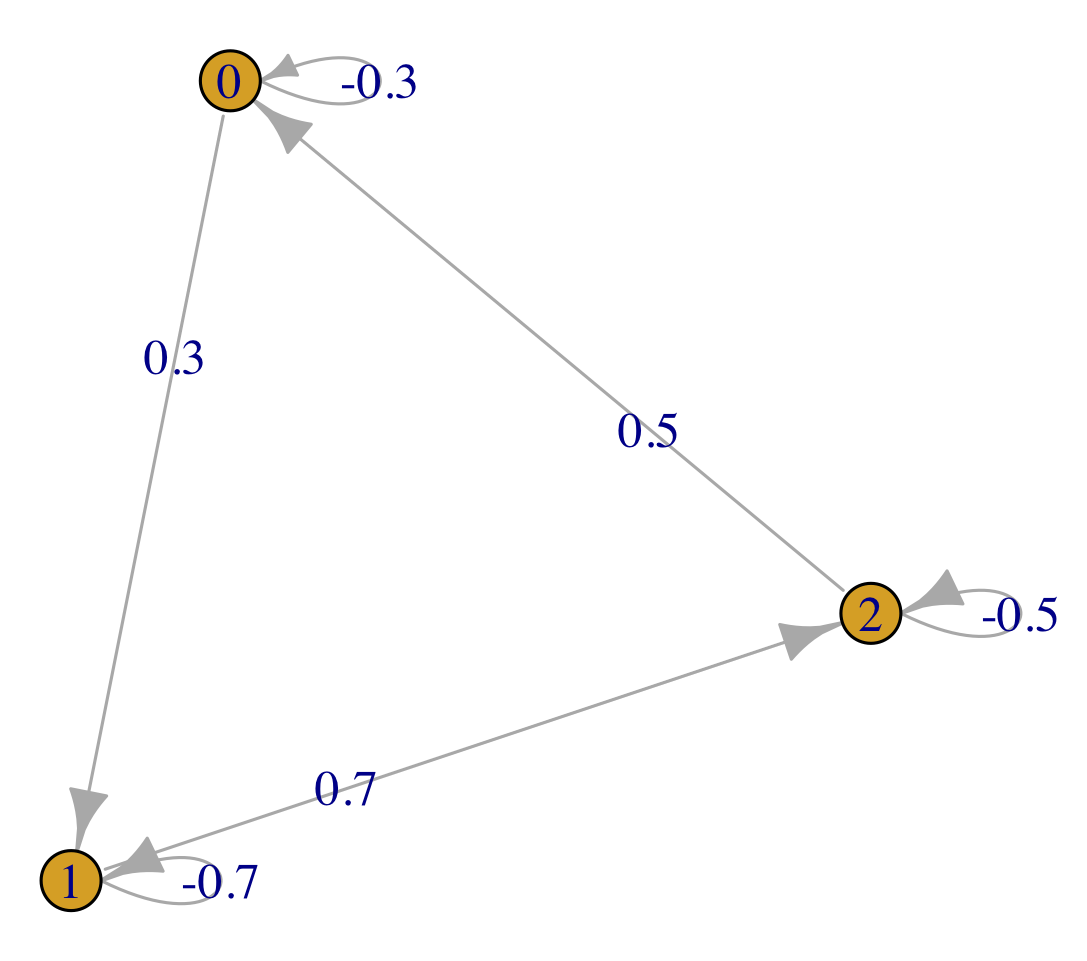
\includegraphics[scale=0.8]{gambar/contoh_ctmc_plot.png}
    \end{center}
\end{frame}

\begin{frame}[fragile]{Simulasi CTMC di R}
    Untuk mensimulasikan CTMC di R, tentukan banyaknya transisi yang ingin disimulasikan,
\begin{minted}{r}
mc2_n <- 10
\end{minted}
    kemudian gunakan fungsi \verb|rctmc| seperti berikut,
\begin{minted}{r}
set.seed(456)
mc2_sim <- rctmc(n = mc2_n, ctmc = mc2_obj,
                 initDist = c(1, 0, 0))
\end{minted}
    yaitu misalnya dengan \textit{initial distribution} (distribusi awal) atau distribusi untuk \(X(0)\) sebagai berikut:
    \[\text{Pr}\brackets{X(0) = 0} = 1, \quad
    \text{Pr}\brackets{X(0) = 1} = 0, \quad
    \text{Pr}\brackets{X(0) = 2} = 0\]
    Hasil simulasi terdiri dari riwayat \textit{state} di \verb|mc2_sim[[1]]|,
\begin{verbatim}
"0" "1" "2" "0" "1" "2" "0" "1" "2" "0" "1"
\end{verbatim}
    dan \textit{transition times} di \verb|mc2_sim[[2]]|,
\begin{verbatim}
0.00000   6.90131  7.23002  8.90053 13.01417 15.74230
16.34644 19.32979 19.96335 22.32489 23.27924
\end{verbatim}
\end{frame}

\begin{frame}[fragile]{Plot Hasil Simulasi CTMC di R}
    Dengan sedikit kode, hasil simulasi CTMC bisa ditampilkan di R (dilampirkan di \textit{slide} selanjutnya).
\begin{minted}{r}
mc2_sim_factors <- factor(mc2_sim[[1]],
                          levels = mc2_states)
mc2_sim_int <- as.integer(mc2_sim_factors)
plot(x = mc2_sim[[2]],
     y = mc2_sim_int,
     xlab = "Waktu (kontinu)",
     ylab = "State",
     main = "Simulasi CTMC",
     yaxt = "n")
axis(2, at = 1 : length(mc2_states), labels = mc2_states)
\end{minted}
\end{frame}

\begin{frame}{Plot Hasil Simulasi CTMC di R}
    \begin{center}
        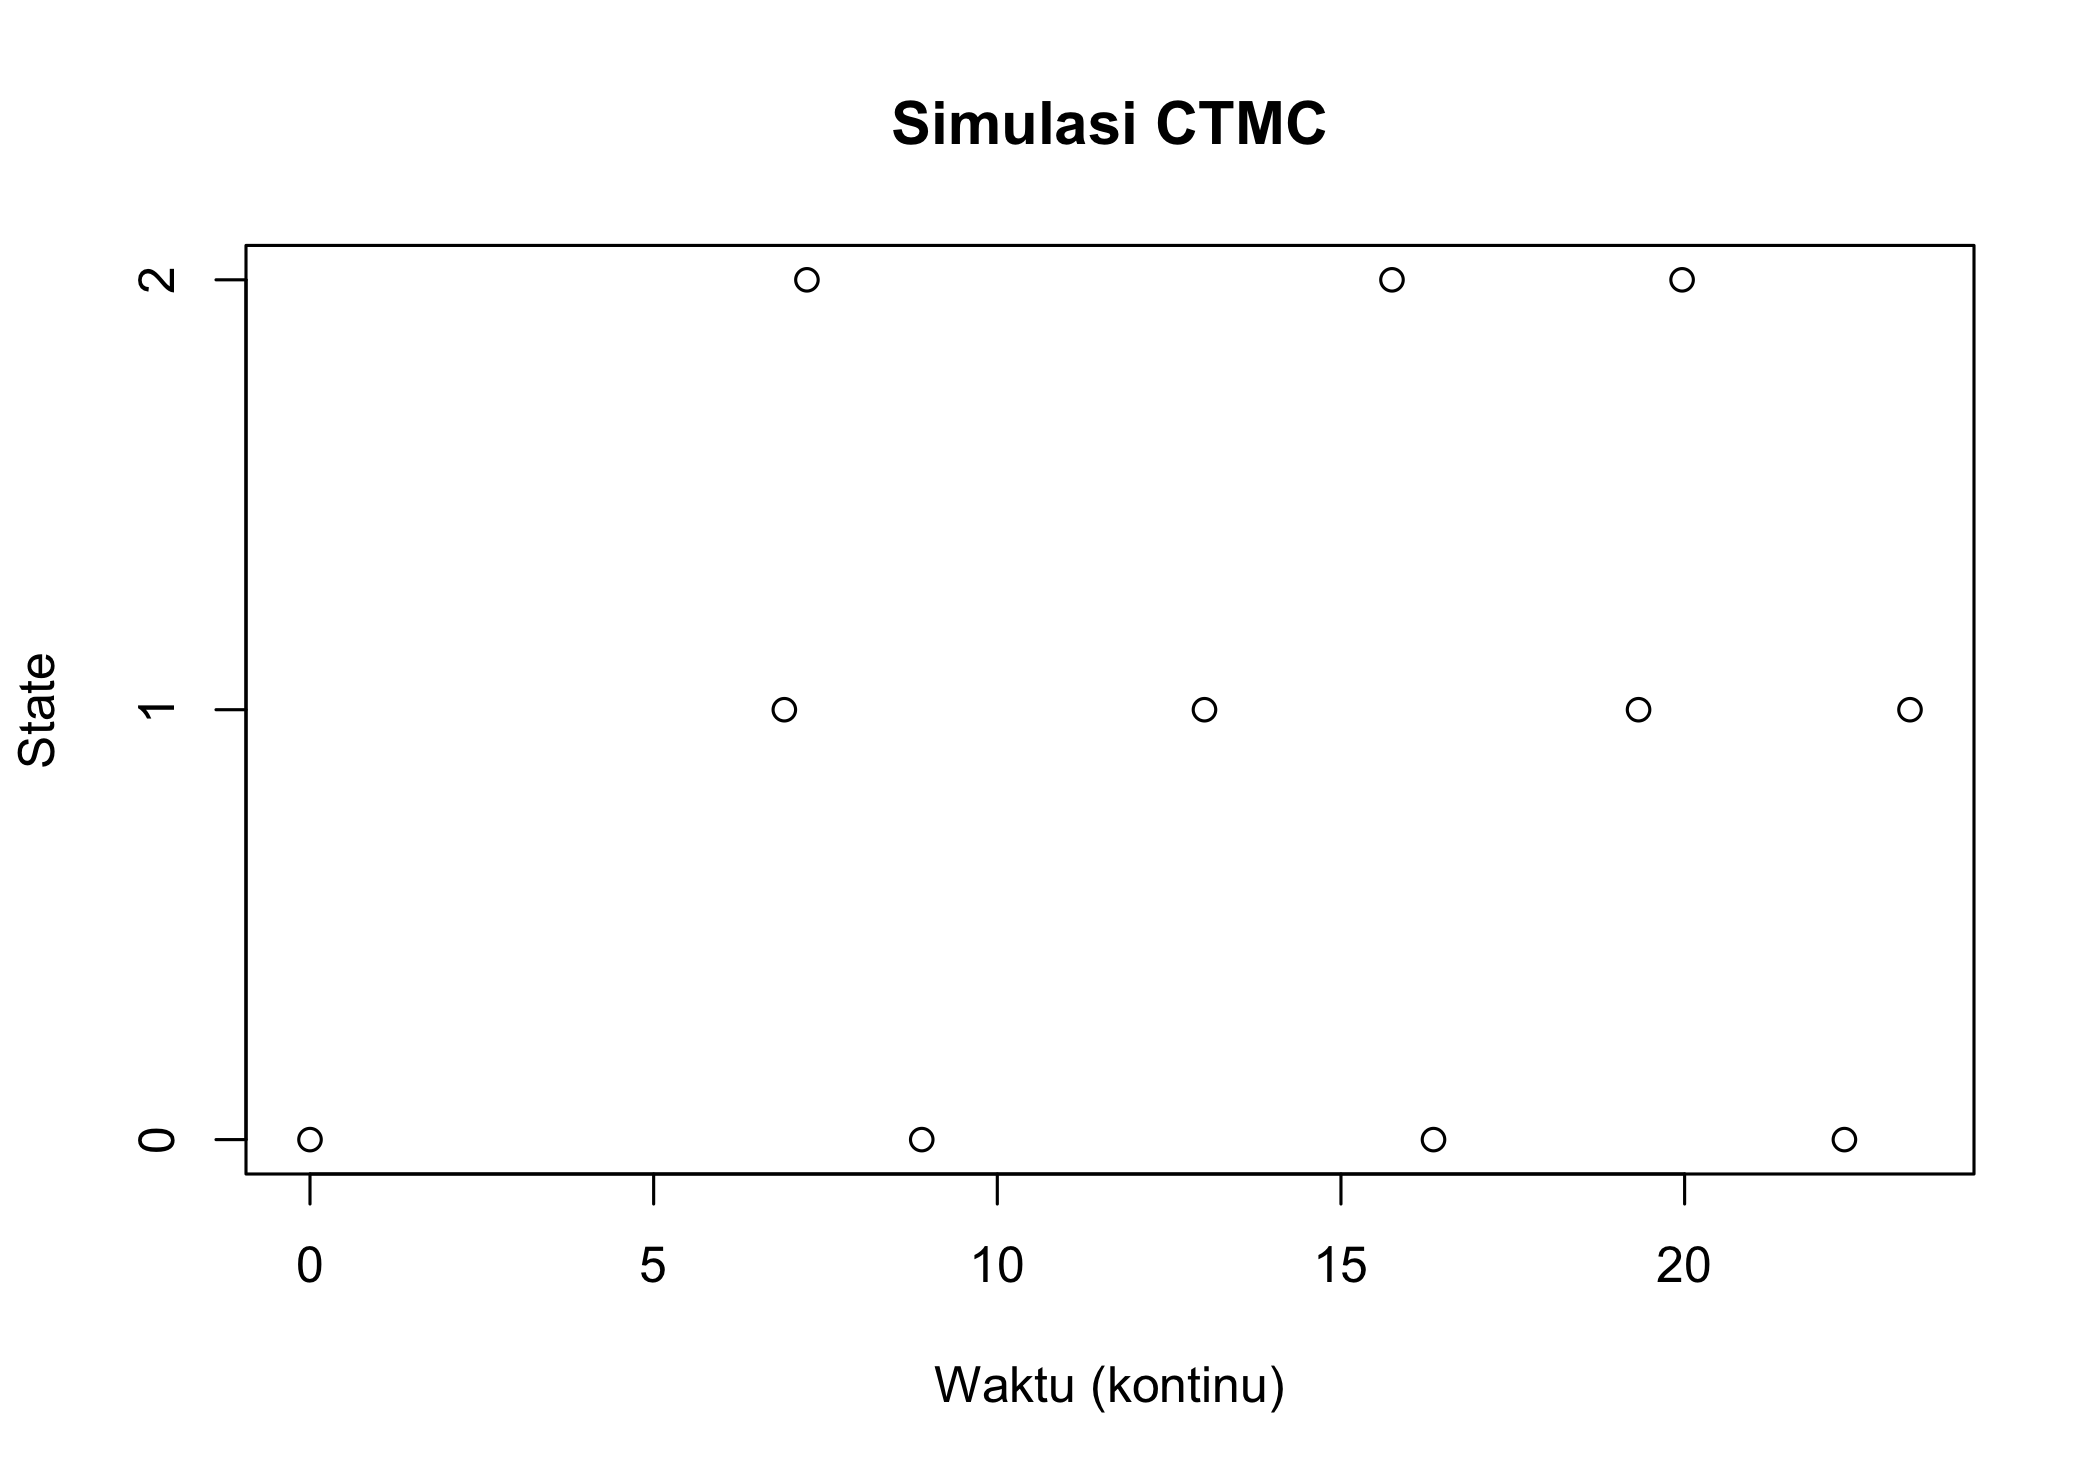
\includegraphics[scale=0.6]{gambar/contoh_ctmc_simulasi.png}
    \end{center}
\end{frame}

\begin{frame}[fragile]{Probabilitas Jangka Panjang CTMC di R}
    Di R, kita dapat menghitung probabilitas jangka panjang \(p_i\) untuk tiap \textit{state} \(i \in S\) dari CTMC dengan
\begin{minted}{r}
steadyStates(mc2_obj)
\end{minted}
    Hasil:
\begin{verbatim}
0            1            2
0.4929577+0i 0.2112676+0i 0.2957746+0i
\end{verbatim}
    artinya,
    \[p_0 \approx 0.4929577, \quad p_1 \approx 0.2112676, \quad p_2 \approx 0.2957746\]
\end{frame}

\begin{frame}[fragile]{Perpangkatan Matriks di R}
    Kita bisa menghitung \(e^A\) di R dengan \textit{package} \verb|expm|
\begin{minted}{r}
# install kalau belum
#install.packages("expm")

library("expm")
\end{minted}
    Untuk menghitung \(e^{Qt}\), pilih nilai \(t\), misalnya \(t = 5\), lalu tulis
\begin{minted}{r}
expm(mc2_Q * 5)
\end{minted}
    Hasilnya juga berupa matriks, dalam hal ini matriks \(P(t) = \pars{P_{ij}(t)}_{i,j\in S}\) ketika \(t=5\):
\begin{verbatim}
          [,1]      [,2]      [,3]
[1,] 0.4934934 0.2211127 0.2853939
[2,] 0.4756564 0.1986765 0.3256671
[3,] 0.5044230 0.2038528 0.2917242
\end{verbatim}
    Perhatikan bahwa hasil-hasil di kolom ke-\(i\) cukup mirip dengan nilai \(p_i\). Semakin besar nilai \(t\), semakin mendekati; karena itulah \(p_i\) disebut "probabilitas jangka panjang".
\end{frame}

\begin{frame}{Iklan (3): Kuliah Model Stokastik 1}
    Asal-usul rumus \(P(t) = e^{Qt}\) untuk matriks fungsi transisi dari CTMC memang tidak dijelaskan di sini. Rumus itu adalah solusi untuk persamaan-persamaan Kolmogorov, kebetulan berupa sistem persamaan diferensial, yang dibahas di kuliah Model Stokastik 1 (3 SKS), bisa diambil di semester depan apabila tertarik, di samping mempelajari DTMC dan proses Poisson. \\[0.5em]
    
    Kasus khusus CTMC yang cukup sering diterapkan di teori antrian adalah \textit{birth-death process}, yang kita bahas selanjutnya.
\end{frame}

\subsection{\textit{Birth-Death Process}}

\begin{frame}{Kasus Khusus CTMC: \textit{Birth-Death Process}}
    \textit{Birth-death process} (BDP) bisa didefinisikan sebagai CTMC \(\braces{X(t); \, t \ge 0 }\) dengan \textit{state space} \(S = \braces{0, 1, 2, \dots}\) dan transisi dari \textit{state} \(i\) ke \textit{state} \(j\) yang mungkin hanyalah
    \begin{itemize}
        \item \(j = i+1\), yang disebut \textit{birth} atau "kelahiran"; dan
        \item \(j = i-1\), yang disebut \textit{death} atau "kematian"
    \end{itemize}
    Karena BDP berupa CTMC, \textit{transition time} (durasi menetap di \textit{state} tertentu sebelum melakukan transisi) untuk kelahiran ataupun kematian berdistribusi eksponensial, bisa ditulis
    \begin{itemize}
        \item \(T_i^{(b)} \sim \text{Exp}\pars{\lambda_i}\), untuk kelahiran menjadi \(j = i+1\), dan
        \item \(T_i^{(d)} \sim \text{Exp}\pars{\mu_i}\), untuk kematian menjadi \(j = i-1\)
    \end{itemize}
    Dalam teori antrian, "kelahiran" diartikan sebagai kedatangan pelanggan dan "kematian" diartikan sebagai kepergian pelanggan, karena \textit{state} \(X(t)\) diartikan sebagai banyaknya pelanggan pada waktu \(t\).
\end{frame}

\begin{frame}{Diagram Transisi BDP dan \textit{Flow Balance}}
    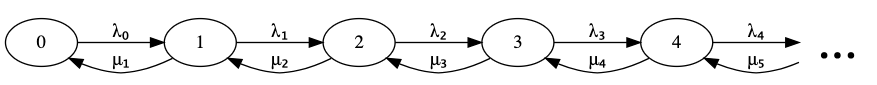
\includegraphics[scale=0.5]{gambar/diagram_transisi_antrian.png}
    Ingat kembali diagram di atas, yang sebenarnya adalah diagram transisi untuk BDP. Untuk menentukan \textbf{probabilitas jangka panjang} berada di \textit{state} \(n\), misal dinotasikan \(p_n\), biasa digunakan konsep \textit{flow balance}, yaitu
    \[\pars{\text{keluar dari \textit{state} } n} = \pars{\text{masuk ke \textit{state} } n}\]
    Untuk \(n = 0\), diperoleh
    \[\lambda_0 p_0 = \mu_1 p_1\]
    dan untuk \(n \ge 1\), diperoleh
    \[ \lambda_n p_n + \mu_n p_n = \lambda_{n-1} p_{n-1} + \mu_{n+1} p_{n+1} \]
    Perhatikan bahwa dalam \textbf{\textit{balance equations}} di atas, tiap \textit{state transition rate}, baik \(\lambda_i\) maupun \(\mu_i\), dikalikan oleh \(p_i\) dengan indeks yang sama.
\end{frame}

\begin{frame}{Solusi \textit{Balance Equations} untuk \(p_n, \, n \ge 1\)}
    Kedua persamaan bisa ditulis menjadi seperti berikut.
    \begin{align*}
        p_1 &= \frac{\lambda_0}{\mu_1} \\
        p_{n+1} &= \frac{\lambda_n + \mu_n}{\mu_{n+1}}p_n - \frac{\lambda_{n-1}}{\mu_{n+1}}p_{n-1}, \quad n \ge 1
    \end{align*}
    Sehingga, ketika \(n = 1\),
    \[p_2 = \frac{\lambda_1 + \mu_1}{\mu_2}p_1 - \frac{\lambda_0}{\mu_2}p_0 = \frac{\lambda_1 \lambda_0}{\mu_2 \mu_1} p_0\]
    Ketika \(n = 2\),
    \[p_3 = \frac{\lambda_2 + \mu_2}{\mu_3}p_2 - \frac{\lambda_1}{\mu_3}p_1 = \frac{\lambda_2 \lambda_1 \lambda_0}{\mu_3 \mu_2 \mu_1} p_0\]
    Muncul pola berikut untuk \(n \ge 1\) (bisa dibuktikan dengan induksi matematika)
    \[\boxed{
        p_n = \frac{\lambda_{n-1} \cdots \lambda_0}{\mu_n \cdots \mu_1} p_0 = p_0 \prod_{i=1}^{n} \frac{\lambda_{i-1}}{\mu_i}
    }\]
\end{frame}

\begin{frame}{Solusi \textit{Balance Equations} untuk \(p_0\)}
    Kita tinggal menentukan \(p_0\). Berdasarkan sifat probabilitas,
    \[\sum_{n=0}^{\infty} p_n = 1\]
    sehingga
    \begin{align*}
        1 &= p_0 + \sum_{n=1}^{\infty} p_n = p_0 + \sum_{n=1}^{\infty} \brackets{p_0 \prod_{i=1}^{n} \frac{\lambda_{i-1}}{\mu_i}} = p_0 + p_0 \sum_{n=1}^{\infty} \prod_{i=1}^{n} \frac{\lambda_{i-1}}{\mu_i} \\
        &= p_0 \pars{1 + \sum_{n=1}^{\infty} \prod_{i=1}^{n} \frac{\lambda_{i-1}}{\mu_i}}
    \end{align*}
    sehingga
    \[\boxed{
        p_0 = \pars{1 + \sum_{n=1}^{\infty} \prod_{i=1}^{n} \frac{\lambda_{i-1}}{\mu_i}}^{-1}
    }\]
\end{frame}

\begin{frame}{\textit{Instantaneous Rate Matrix} \(Q\) untuk BDP}
    Karena BDP tergolong CTMC, BDP memiliki \textit{instantaneous rate matrix} \(Q = \pars{Q_{ij}}_{i,j\in S}\) dan juga \textit{state transition rate} \(v_i = \lambda_i + \mu_i\) karena
    \[\text{min}\braces{T_i^{(b)}, T_i^{(d)}} \sim \text{Exp}\pars{\lambda_i + \mu_i}\]
    Selain itu, karena transisi yang mungkin hanyalah \(j=i+1\) dan \(j=i-1\), probabilitasnya proporsional dengan \textit{state transition rate}, seperti berikut:
    \[P_{i,i+1} = \frac{\lambda_i}{\lambda_i + \mu_i}, \quad P_{i,i-1} = \frac{\mu}{\lambda_i + \mu_i}\]
    Perhatikan bahwa, untuk tiap \(i \ge 1\),
    \begin{align*}
        q_{i,i+1} &= v_i P_{i,i+1} = \pars{\lambda_i + \mu_i} \pars{\frac{\lambda_i}{\lambda_i + \mu_i}} = \lambda_i \\
        q_{i,i-1} &= v_i P_{i,i-1} = \pars{\lambda_i + \mu_i} \pars{\frac{\mu}{\lambda_i + \mu_i}} = \mu_i \\
        q_{i,j} &= v_i P_{ij} = \pars{v_i} (0) = 0, \quad j \notin \braces{i-1, i, i+1} \\
        q_{i,i} &= -\pars{q_{i,i+1} + q_{i,i-1}} = -\pars{\lambda_i + \mu_i}
    \end{align*}
\end{frame}

\begin{frame}{\textit{Instantaneous Rate Matrix} \(Q\) untuk BDP}
    Ketika \(i=0\), transisi hanya mungkin ke \(j=1\) karena tidak boleh ke diri sendiri (sifat CTMC) dan tidak mungkin menurun lagi (\(\mu_0 = 0\)), sehingga
    \[P_{01} = 1, \quad q_{01} = v_0 P_{01} = v_0 = \lambda_0 + \mu_0 = \lambda_0, \quad q_{00} = -q_{01} = -\lambda_0\]
    Dengan demikian, bentuk umum \textit{instantaneous rate matrix} untuk sembarang BDP bisa ditulis
    \[Q = \begin{pmatrix}
        -\lambda_0 & \lambda_0 & 0 & 0 & 0 & \cdots \\
        \mu_1 & -\pars{\lambda_1 + \mu_1} & \lambda_1 & 0 & 0 & \cdots \\
        0 & \mu_2 & -\pars{\lambda_2 + \mu_2} & \lambda_2 & 0 & \cdots \\
        0 & 0 & \mu_3 & -\pars{\lambda_3 + \mu_3} & \lambda_3 & \cdots \\
        \vdots & \vdots & \vdots & \vdots & \vdots & \ddots
    \end{pmatrix}\]
    yaitu matriks tridiagonal. Dengan matriks ini, simulasi BDP di R bisa saja dilakukan sebagaimana simulasi CTMC di R.
\end{frame}

% simulasi dengan finite state saja agak aneh, apalagi simulasi CTMC sudah ditunjukkan sebelumnya...
%\begin{frame}[fragile]{Simulasi BDP di R}
    %tes
%\end{frame}

\begin{frame}{Kasus Khusus BDP}
    Terdapat dua kasus khusus BDP yang umum dikenal, yaitu
    \begin{enumerate}
        \item \textit{Pure birth process} ketika hanya ada "kelahiran" saja, yaitu ketika tidak ada "kematian": \(\mu_i = 0\) untuk tiap \(i \in S\)
        \begin{itemize}
            \item \textbf{Proses Poisson} dengan \textit{rate} \(\lambda\) adalah \textit{pure birth process} dengan \(\lambda_i = \lambda\).
        \end{itemize}
        \item \textit{Pure death process} ketika hanya ada "kematian" saja, yaitu ketika tidak ada "kelahiran": \(\lambda_i = 0\) untuk tiap \(i \in S\)
    \end{enumerate}
\end{frame}

\begin{frame}{Iklan (4): Kuliah Model Stokastik 1}
    Tidak hanya proses Poisson, terdapat beberapa variasi BDP lainnya, termasuk variasi \textit{pure birth process} dan variasi \textit{pure death process}. Itu semua dipelajari di kuliah Model Stokastik 1 (3 SKS), termasuk berbagai contoh pemodelan dan aplikasinya, demikian juga untuk DTMC dan CTMC secara umum. Apabila tertarik, silakan ambil kuliah Model Stokastik 1 di semester genap bersama mahasiswa prodi S1 Statistika dan/atau S1 Ilmu Aktuaria. \\[0.5em]

    (Ini adalah iklan terakhir untuk kuliah Model Stokastik 1. Silakan dipertimbangkan.) \\[0.5em]

    Sangat dekat dengan konsep BDP adalah model antrian M/M/1 dan M/M/c, yaitu tujuan akhir pembahasan di sini. Sebelum itu, berikut ini kita bahas tentang konsep antrian secara umum.
\end{frame}

\subsection{Antrian dan Notasinya}

\begin{frame}{Konsep dasar teori antrian}
    Tiap model yang dibahas di teori antrian terdiri dari \textbf{antrian} dan \textbf{sistem}. Semua peserta secara umum disebut \textbf{pelanggan}.
    \begin{itemize}
        \item "Sistem" terdiri dari tempat mengantri (disebut "antrian") dan tempat pelayanan.
        \item Dalam suatu sistem, bisa saja ada pelanggan yang sedang dilayani dan juga ada pelanggan yang masih mengantri menunggu dilayani (masih di antrian).
        \item Banyaknya pelanggan yang biasa dihitung adalah \textbf{banyaknya pelanggan di sistem} secara keseluruhan, tidak hanya yang ada di antrian.
        \item Alurnya adalah: (1) masuk ke dalam sistem; (2) mengantri apabila tempat pelayanan masih penuh; (3) langsung dilayani apabila sudah di depan antrian dan ada tempat pelayanan yang kosong; lalu (4) meninggalkan sistem ketika pelayanan sudah selesai.
        \item Tempat pelayanan bisa terdiri dari satu atau sejumlah \textbf{\textit{server}} (pelayan), masing-masing bisa melayani satu pelanggan.
    \end{itemize}
\end{frame}

\begin{frame}{Penamaan sistem antrian}
    Suatu model antrian atau sistem antrian biasa dilambangkan misalnya A/B/X/Y/Z, yang artinya berturut-turut (sesuai posisi) adalah
    \begin{enumerate}
        \item A: Pola kedatangan; distribusi \textit{interarrival time} (durasi antara satu kedatangan dengan yang berikutnya)
        \item B: Pola pelayanan; distribusi \textit{service time} (durasi pelayanan; seperti \textit{interarrival time} tetapi untuk kepergian pelanggan)
        \item X: Banyaknya \textit{server} \(\pars{1, 2, \dots, c, \dots, \infty}\)
        \item Y: Kapasitas sistem; maksimum banyaknya pelanggan dalam sistem \(\pars{1, 2, \dots, K, \dots, \infty}\)
        \item Z: \textit{Queue discipline}, yaitu cara memilih pelanggan berikutnya dari antrian untuk dilayani
    \end{enumerate}
    Terkadang, penulisan dipotong, misalnya hanya ditulis A/B/X. Biasanya, dianggap \(Y = \infty\) dan Z = FCFS (\textit{first come first serve;} urutan pelayanan pelanggan dimulai dari yang paling pertama datang).
\end{frame}

\begin{frame}{Aspek-aspek sistem antrian dan notasinya}
    Perhatikan bahwa \textit{subscript} huruf \(q\) melambangkan \textit{queue} (antrian). Apabila tidak ada \textit{subscript} \(q\), maka ukuran tersebut adalah untuk sistem.
    \begin{itemize}
        \item \(\lambda\): \textit{rate} rata-rata untuk kedatangan
        \item \(S\): variabel acak durasi pelayanan
        \item \(\mu = 1/\text{E}\brackets{S}\): \textit{rate} rata-rata untuk pelayanan
        \item \(c\): banyaknya \textit{server}
        %\item \(K\): kapasitas sistem
        \item \(r = \lambda/\mu\): \textit{offered load}, %(\textit{rate} rata-rata kedatangan beban)
        rata-rata banyaknya \textit{server} "sibuk" (sedang melayani)
        \item \(\rho = \lambda/c\mu\): \textit{traffic intensity} (ukuran kemacetan) atau \textit{utilization}, proporsi waktu \textit{server} sibuk
        \item \(T, T_q\): variabel acak durasi pelanggan di sistem/antrian
        \item \(W, W_q\): rata-rata durasi pelanggan di sistem/antrian
        \item \(N, N_q\): variabel acak banyaknya pelanggan di sistem/antrian
        \item \(L, L_q\): rata-rata banyaknya pelanggan di sistem/antrian
    \end{itemize}
\end{frame}

\begin{frame}{\textit{Little's Law:} \(L = \lambda W\) dan \(L_q = \lambda W_q\)}
    \begin{itemize}
        \item \textit{Little's Law} menyatakan bahwa rata-rata banyaknya pelanggan di sistem sama dengan \textit{rate} rata-rata untuk kedatangan dikali dengan rata-rata durasi pelanggan di sistem.
        \[L = \lambda W\]
        \item Berlaku juga khusus antriannya daripada untuk sistem secara keseluruhan, yaitu
        \[L_q = \lambda W_q\]
        \item Bisa dianalogikan dengan rumus fisika \(s = vt\)
        \item Contoh: \textbf{mengantri lulus SD}. Jika sekitar \(\lambda = 30\) siswa/tahun masuk suatu SD (mulai dari kelas 1 SD), dan rata-rata durasi sekolah SD adalah \(W = 6\) tahun (ingat ada akselerasi dan tidak naik kelas), maka rata-rata banyaknya siswa yang sedang bersekolah di SD tersebut adalah
        \[L = \lambda W = \pars{30 \text{ siswa/tahun}}\pars{6 \text{ tahun}} = 180 \text{ siswa}\]
    \end{itemize}
\end{frame}

\begin{frame}{Rumus-rumus umum untuk \(G/G/c\)}
    \(G/G/c\) adalah sistem antrian dengan distribusi \textit{interarrival time} dan distribusi \textit{service time} yang umum \textit{(general)} dengan \(c\) \textit{server}. Untuk \(G/G/c\), berlaku
    \begin{itemize}
        \item \textit{Little's law:} \(L=\lambda W\) dan \(L_q = \lambda W_q\)
        \item \(T = T_q + S\), durasi pelanggan di sistem adalah durasi mengantri ditambah durasi dilayani
        \item \(W = W_q + 1/\mu\), ekspektasi dari persamaan di atas
        \item \(L = L_q + r\),
        % dari persamaan di atas dan kedua rumus \textit{Little's law}
        dengan substitusi persamaan di atas ke \textit{Little's law}
        \item \(r = \lambda/\mu\)
        \item \(\rho = \lambda/c\mu\)
    \end{itemize}
    Ketika \(c=1\), yaitu untuk \(G/G/1\), juga berlaku
    \begin{itemize}
        \item \(p_0 = 1 - \rho\)
        \item \(L = L_q + \rho\), karena \(r = \rho\) ketika \(c=1\)
    \end{itemize}
\end{frame}

\begin{frame}{Notasi dan rumus \textit{bookkeeping} (pencatatan) untuk (simulasi) sistem antrian}
    \begin{itemize}
        \item \(A^{(n)}\): kapan pelanggan ke-\(n\) datang \textit{(arrival)}
        \item \(S^{(n)}\): durasi pelangan ke-\(n\) dilayani \textit{(service)}
        \item \(T^{(n)}\): \textit{interarrival time} atau durasi antar kedatangan ke-\(n\) dengan ke-\((n+1)\), 
        \(T^{(n)} = A^{(n+1)} - A^{(n)}\)
        \item \(U^{(n)}\): kapan pelanggan ke-\(n\) mulai dilayani \textit{(use)}, 
        \(U^{(n+1)} = \text{max}\braces{D^{(n)}, \, A^{(n+1)}}\)
        \item \(D^{(n)}\): kapan pelanggan ke-\(n\) meninggalkan sistem \textit{(departure)}, 
        \(D^{(n)} = U^{(n)} + S^{(n)}\)
        \item \(W_q^{(n)}\): durasi pelanggan ke-\(n\) di antrian (menunggu; \textit{waiting}), 
        \(W_q^{(n)} = U^{(n)} - A^{(n)}\)
        \item \(W^{(n)}\): durasi pelanggan ke-\(n\) di sistem, 
        \(W^{(n)} = W_q^{(n)} + S^{(n)}\)
    \end{itemize}
\end{frame}

\begin{frame}{Antrian sebagai \textit{Birth-Death Process}}
    \begin{itemize}
        \item Beberapa sistem antrian sederhana kebetulan berupa BDP tertentu
        \item Huruf M dalam notasi M/M/X/Y/Z melambangkan sifat Markov atau \textit{memoryless property}, mengindikasikan distribusi eksponensial, berturut-turut dengan \textit{rate} \(\lambda\) dan \(\mu\)
        \item (belum jadi)
    \end{itemize}
\end{frame}

\section{Antrian M/M/c}

\subsection{M/M/c secara umum}

\subsection{Kasus khusus: Antrian M/M/1}

\subsection{Simulasi M/M/c di R}

\subsection{M/M/c di QtsPlus}

\section{Lampiran: Tautan, \textit{GitHub repository}, Referensi}

\begin{frame}{Tautan dan \textit{GitHub repository}}
    Untuk \textit{package} R yang digunakan:
    \begin{itemize}
        \item markovchain: \url{https://github.com/spedygiorgio/markovchain}

        \item queuecomputer: \url{https://github.com/AnthonyEbert/queuecomputer}
        
        \item queueing: \url{https://cran.r-project.org/web/packages/queueing/index.html}
    \end{itemize}

    Tautan lainnya:

    \begin{itemize}
        \item QtsPlus v4.0: \url{https://mason.gmu.edu/~jshortle/fqt5th.html}
        
        \item \textit{GitHub repository} untuk presentasi ini (termasuk kode): \url{https://github.com/BismaBRJ/intro_stokastik_antrian_r_2024/}
    \end{itemize}
\end{frame}

\begin{frame}{Referensi}
    \begin{itemize}
        \item Pinsky, Mark A. \& Karlin, Samuel (2011). \textit{An Introduction to Stochastic Modeling} (edisi ke-2). Elsevier.
        
        \textbf{Untuk:} sebagian besar materi DTMC, proses Poisson, dan CTMC, kecuali contoh dan simulasi dengan R

        \item Shortle, John F.; Thompson, James M.; Gross, Donald; \& Harris, Carl M. (2018). \textit{Fundamentals of Queueing Theory} (edisi ke-5). Wiley. \url{https://mason.gmu.edu/~jshortle/fqt5th.html}
        
        \textbf{Untuk:} sebagian besar materi \textit{birth-death process} dan antrian, termasuk M/M/c, kecuali contoh dan simulasi dengan R

        \textbf{Catatan:} sering disebut buku \textbf{Gross \& Harris} karena merekalah yang menulis edisi pertama
    \end{itemize}
\end{frame}

\end{document}